\chapter{Cónicas y Cuádricas}
\label{C8}
A lo largo del capítulo $\ref{C2}$ estudiamos con detalle el conjunto de puntos que eran anulados por unas aplicaciones muy concretas, a las que llamamos \ti{formas lineales}.

En este capítulo haremos algo parecido, dando un pequeño paso adelante, pues estudiaremos las interesantes propiedades del conjunto de ceros de las llamadas \ti{formas cuadráticas}.

A no ser que establezcamos explícitamente lo contrario, a lo largo de este capítulo trabajaremos con el cuerpo de los números complejos y el plano proyectivo complejo $\proy(\C^3)=\proy^2$. 

Esto es debido a que, como se verá inmediatamente, trabajaremos con polinomios, siendonos muy útil la posibilidad de aplicar el Teorema Fundamental del Álgebra y sus consecuencias.

El capítulo comienza con una fuerte introducción teórica acerca de formas bilineales y cuadráticas (muy susceptible de haber sido olvidada), e indispensable para comprender en profundidad los resultados centrales del capítulo (razón por la cual se ha decidido incluirla aquí y no en un apéndice dedicado).

\section{Conceptos Previos. Formas Bilineales y Cuadráticas}
A lo largo de este capítulo estudiaremos las llamadas \ti{cuádricas}. Para poder definir de forma rigurosa este concepto, necesitamos recordar (o introducir) algunas nociones importantes más propias del álgebra lineal.
\subsection{Formas Bilineales}
Sea $E$ un espacio vectorial arbitrario de dimensión $n$. (Normalmente trabajaremos con $\C^n$).
\begin{defi}[Forma Bilineal]
	\label{C8_def_formaBilineal}
	Llamamos \ti{formas bilineales} a las aplicaciones de la forma \[\begin{array}{cc}f:&E\times E\to\K\\
	& (u,v)\mapsto f(u,v)\end{array}\]
	Donde $f$ es ``lineal respecto de ambas componentes''. Es decir, dado un par $(u,v)\in E\times E$, se verifica:
	\begin{enumerate}
		\item Linealidad respecto de la primera componente: \[f(\alpha u_1,\beta u_2, v)=\alpha f(u_1,v)+\beta f(u_2,v)\]
		\item Linealidad respecto de la segunda componente:
		\[f(u,\alpha v_1 +\beta v_2)=\alpha f(u,v_1)+\beta f(u,v_2)\]
	\end{enumerate}
\end{defi}
En este punto es fructífero recordar que una aplicación lineal queda totalmente determinada por las imágenes de los vectores de una base de su espacio vectorial de partida.

Este resultado daba lugar a la idea caracterizar cada aplicación lineal $f$ por una matriz, a la que llamábamos \ti{matriz asociada a $f$}.

Tratemos de trasladar esta idea al ámbito de las formas bilineales.
\subsubsection{Matriz Asociada a una Forma Bilineal}
Fijemos una base $\mc{B}:=\{e_1,\dots,e_n\}$ del espacio vectorial $E$.

Veamos cuál es la imagen del par $(u,v)$ por una forma bilineal arbitraria $f$. Para ello, escribiremos los vectores $u$ y $v$ como combinación lineal de la base $\mc{B}$ y aplicaremos las propiedades de bilinealidad (definición \ref{C8_def_formaBilineal})
\[f(u,v)=f\left(\sum_{i=1}^{n}a_ie_i,\sum_{j=1}^{n}b_je_j\right)=\sum_{i=1}^{n}a_i\left(\sum_{j=1}^{n}f(e_i,e_j)b_j\right)\]
Podemos interpretar el interior del paréntesis como un producto de matrices (matriz fila por matriz columna). Haciendo esto obtenemos la siguiente expresión, más compacta (los corchetes son sólo notacionales).
\[f(u,v)=\sum_{i=1}^{n}a_i\left[\begin{pmatrix}
f(e_i, e_1) & 
\cdots &
f(e_i, e_n)
\end{pmatrix}\begin{pmatrix}
b_1 & \cdots & b_n
\end{pmatrix}^t\right]\]
Por comodidad notacional, a la matriz columna que representa las coordenadas de $v$ respecto de $\mc{B}$ será denotado por $Y$. Análogamente, llamaremos $X$ a la matriz columna que representará las coordenadas de $u$ respecto de $\mc{B}$.

Con esta notación (y reordenando por conveniencia los corchetes) nos queda:
\[f(u,v)=\left[\sum_{i=1}^{n}a_i\begin{pmatrix}
f(e_i, e_1) & 
\cdots &
f(e_i, e_n)
\end{pmatrix}\right]Y\]
Como hicimos antes, podemos interpretar la suma anterior de manera matricial (las comprobaciones de dejan al lector)
\[f(u,v)=\begin{pmatrix}
a_1 & \cdots & a_n
\end{pmatrix}\begin{pmatrix}
f(e_1, e_1) & \cdots & f(e_1,e_n)\\
\vdots & \ddots & \vdots\\
f(e_n,e_1) & \cdots & f(e_n,e_n)
\end{pmatrix}Y\]
Usando nuestras notaciones habituales y denotando por $M$ a la matriz cuadrada obtenemos:
\begin{equation}
\label{C8_eq_ecuacionMatricialBilineal}
f(u,v)=X^tMY
\end{equation}
A la matriz $M$ de la ecuación \eqref{C8_eq_ecuacionMatricialBilineal} se la llama \ti{matriz asociada a la forma bilineal $f$}.

Se ve inmediatamente por la ecuación \eqref{C8_eq_ecuacionMatricialBilineal} que si dos formas bilineales $f$ y $g$ tienen a $M$ por matriz asociada, estas son necesariamente la misma aplicación.

Esto quiere decir que una forma bilineal $f$ queda totalmente determinada por su matriz asociada, es decir, por las imágenes de los pares de vectores $(e_i,e_j)$ donde $i,j\in\{1,\dots,n\}$.

\begin{obs}[Lema de la Correspondencia]
	\label{C8_obs_correspondencia}
	Es claro que a lo largo de este proceso hemos probado que, \tb{fijada una base} $\mc{B}$ de $E$, toda forma bilineal $f$ está asociada a una única matriz $M$.
	
	Además, el recíproco también es cierto, fijada una base, toda matriz cuadrada es la asociada de una única forma bilineal.
	
	La prueba de este hecho consiste símplemente en definir una forma bilineal $f$ de manera que la imagen de un par de la forma $(e_i,e_j)$ se corresponda con el coeficiente $a_{ij}$ de la matriz dada. 
\end{obs}
\subsection{Formas Cuadráticas}
Introducidos ya los aspectos generales de las formas bilineales, pasemos a definir la noción de \ti{forma cuadrática}.
\begin{defi}[Forma Cuadrática]
	Una aplicación $\Phi$ se dice \ti{forma cuadrática} si es de la forma:
	\[\begin{array}{cc}
	\Phi: & E\to \K\\
	& x\mapsto f(x,x)
	\end{array}\]
	donde $f$ es una forma bilineal.
\end{defi}
Es claro que, fijada una base, las formas cuadráticas cumplen la siguiente ecuación matricial:
\begin{equation}
\label{C8_eq_ecuacionCuadraticas}
	\Phi(x)=X^tMX
\end{equation}
Una propiedad agridulce de las formas cuadráticas es que pueden estar asociadas a varias formas bilineales, tal y como muestra el siguiente ejemplo.
\begin{exa}[Varias Formas Bilineales Asociadas]
	Sean las formas bilineales de matrices asociadas:
	\[f\equiv\begin{pmatrix}
	1 & 4\\
	2 & 2
	\end{pmatrix}\qquad g\equiv\begin{pmatrix}
	1 & 3\\
	3 & 2
	\end{pmatrix}\]
	Comprobemos que ambas formas bilineales tienen la misma forma cuadrática asociada.
	\[\Phi_f(x)=\begin{pmatrix}
	x_1 & x_2
	\end{pmatrix}\begin{pmatrix}
	1 & 4\\
	2 & 2
	\end{pmatrix}\begin{pmatrix}
	x_1\\
	x_2
	\end{pmatrix}=x_1^2+6x_1x_2+2x_2^2\]
	\[\Phi_g(x)=\begin{pmatrix}
	x_1 & x_2
	\end{pmatrix}\begin{pmatrix}
	1 & 3\\
	3 & 2
	\end{pmatrix}\begin{pmatrix}
	x_1\\
	x_2
	\end{pmatrix}=x_1^2+6x_1x_2+2x_2^2\]
\end{exa}
Decimos que esta propiedad es ``agridulce'', porque por una parte es más bonito que haya una correspondencia ``limpia'' entre formas bilineales y formas cuadrátricas. Sin embargo, las propiedades que vienen a continuación compensan con creces esto último. Antes de poder presentarlas, necesitamos una pequeña definición.
\begin{defi}[Formas Bilineales Simétricas y Antisimétricas]
	\label{C8_def_simetricaAntisimetrica}
	Decimos que una forma bilineal $f$ es \ti{simétrica} si su matriz asociada es simétrica. Análogamente, $f$ será \ti{antisimétrica} (o \ti{alternada}) si su matriz asociada es antisimétrica.
\end{defi}
Nótese que en la definición \ref{C8_def_simetricaAntisimetrica} hablamos de la matriz asociada a una forma bilineal como si solo hubiera una y no muchas (una por cada base fijada).

De esta forma, en primera instancia, uno podría pensar que es posible que hubiera dos bases; $\mc{B}$ y $\overline{\mc{B}}$, de manera que la matriz asociada a cierta forma bilineal $f$ fuera simétrica respecto de la base $\mc{B}$ y antisimétrica respecto de $\overline{\mc{B}}$.

Los siguientes lemas demuestran que esto es imposible. Más aún, veremos que  si la matriz asociada a una forma bilineal $f$ es simétrica respecto de una base $\mc{B}$, lo será también respecto de cualquier otra base $\overline{\mc{B}}$.

De esta forma, podemos decir que la simetría o antisimetría de una forma bilineal es una propiedad intrínseca de la aplicación y no del modo en que la miramos.
\begin{lem}[Caracterización de las Formas Bilineales Simétricas]
	\label{C8_lem_caracterizacionSimetria}
	$f$ es una forma bilineal simétrica si y solo si se verifica que \[f(x,y)=f(y,x)\]
\end{lem}
\begin{proof}
	Si $f$ es una forma bilineal simétrica entonces \[f(x,y)=X^tMY=(X^tMY)^t=Y^tM^tX=Y^tMX=f(y,x)\]
	Recíprocamente, si $f(x,y)=f(y,x)$ es claro que \[a_{ij}:=f(e_i,e_j)=f(e_j,e_i)=:a_{ji}\]
	Que es la definición de ser una matriz simétrica.
\end{proof}
\begin{lem}[Caracterización de las Formas Bilineales Antisimétricas]
	$f$ es una forma bilineal simétrica si y solo si se verifica que \[f(x,y)=-f(y,x)\]
\end{lem}
\begin{proof}
	Se deja como ejercicio al lector. Es totalmente análoga a la del lema \ref{C8_lem_caracterizacionSimetria}. 
\end{proof}
Demostrados los lemas anteriores, que quizá nos hayan roto un poco el discurrir de la teoría, veamos cuál es su verdadera utilidad.

Los siguientes resultados, elementales, pero cruciales, nos hacen ver que, de alguna manera, hay una forma bilineal canónica asociada a cada forma cuadrática. 
\begin{lem}[Formas Cuadráticas Idénticamente Nulas]
	\label{C8_lem_antisimetricaNula}
	Si $\Phi$ es una forma cuadrática asociada a una forma bilineal antisimétrica, entonces $\Phi$ es idénticamente nula.
\end{lem}
\begin{proof}
	Por la ecuación \eqref{C8_eq_ecuacionCuadraticas} sabemos que:
	\[\Phi(x)=X^tMX\in\K\]
	Tenemos que tratar de aplicar en algún sitio que la matriz $M$ es antisimétrica, para lo cual, lo ideal es trasponer en angún lugar.
	
	Como $X^tMX$ es un simple número, coincide con su traspuesto, lo cual nos arroja:
	\[\Phi(x)=X^tMX=(X^tMX)^t=X^tM^tX=-X^tMX=-\Phi(x)\]
	Por ende, $2\Phi(x)=0$, de lo que se desprende que $\Phi(x)=0$ para cualquier $x\in E$.
\end{proof}
\begin{lem}
	\label{C8_lem_descomposicion}
	Sea $M$ una matriz cuadrada, admite una descomposición como suma de una matriz simétrica y otra antisimétrica.
	\[M= M_s+M_a\]
	Además
	\[\begin{array}{cc}
	M_s=\frac{1}{2}(M+M^t)\qquad &\qquad M_a=\frac{1}{2}(M-M^t)
	\end{array}\]
	En términos de formas bilineales; toda forma bilineal puede descomponerse como suma de una forma bilineal simétrica y una forma bilineal antisimétrica.
\end{lem}
\begin{proof}
	Se deja como ejercicio al lector (es una comprobación trivial).
\end{proof}
\begin{obs}[Redundancia de la Parte Antisimétrica]
	De los lemas \ref{C8_lem_antisimetricaNula} y \ref{C8_lem_descomposicion} se deduce que la parte antisimétrica de una forma bilineal asociada a una forma cuadrática sólo nos aporta ruido y confusión.
	
	En efecto, dada una forma cuadrática $\Phi$ tenemos que
	\begin{multline}\Phi(x)=X^tMX=X^t(M_s+M_a)X=\\=(X^tM_s+X^tM_a)X=X^tM_sX+X^tM_aX=X^tM_sX\end{multline}
	Esto constituye una fábrica de formas bilineales asociadas a una misma forma cuadrática.
	
	El hecho de que esto sea siquiera posible nos lleva a la idea de que sería recomendable deshacernos de esa dichosa parte antisimétrica (ya que es más inútil que un cubo de trapo).
\end{obs}
Si combinamos los lemas \ref{C8_lem_antisimetricaNula} y \ref{C8_lem_descomposicion} obtenemos que, tal y como nos asegura el siguiente resultado, una forma cuadrática está asociada a una única forma bilineal simétrica.
\begin{prop}[Lema de la Correspondencia]
	Dada una forma cuadrática $\Phi$, esta está asociada a una única forma bilineal simétrica $f_p$.
	
	A dicha forma bilineal se le llama ``\ti{forma polar}'' de $\Phi$.
\end{prop}
\begin{proof}
	Es una comprobación inmediata ver que se cumple
	\[\Phi(x+y)=f(x,y)+f(y,x)+\Phi(x)+\Phi(y)\]
	Si $f$ es simétrica se cumple que
	\[f(x,y)=\frac{1}{2}\left(\Phi(x+y)-\Phi(x)-\Phi(y)\right)\]
	Por lo que no solo hemos demostrado la unicidad, sino que también hemos obtenido una expresión explícita de la misma.
\end{proof}
Si esta demostración le ha dejado frío al lector (porque ser chapucera y poco intuitiva), que no se alarme, veremos una múcho más útil y elegante en secciones posteriores. (Ver proposición \ref{C8_prop_Hessiana}).
\subsubsection{Matriz Asociada a una Forma Cuadrática}
Podemos definir (por decreto) el concepto de \ti{matriz asociada a una forma cuadrática} $\Phi$ como la matriz asociada a su forma polar.

Pongamos un ejemplo (muy importante en nuestro contexto) para que estos conceptos se arraiguen más.
\begin{exa}[Forma Cuadrática de Dimensión $3$]
	\label{C8_exa_3forma}
	Como sabemos, fijada una base $\mc{B}$, las formas cuadráticas verifican la ecuación matricial
	\[\Phi(\vec{x})=X^tMX\]
	donde consideramos que $M$ es la matriz (simétrica) asociada a la forma cuadrática. En el caso de estar en un espacio vectorial de tres dimensiones tendremos algo del estilo
	\[\Phi(\vec{x})=\begin{pmatrix}
	x & y & z
	\end{pmatrix}\begin{pmatrix}
	a & h & g\\
	h & b & f\\
	g & f & c
	\end{pmatrix}\begin{pmatrix}
	x\\
	y\\
	z
	\end{pmatrix}\]
	Si desarrollamos esto obtenemos la siguiente expresión (que nos será muy familiar de ahora en adelante)
	\begin{equation}
	\label{C8_eq_polinomio}
	\Phi(\vec{x})=ax^2+by^2+cz^2+2fyz+2gzx+2hxy\end{equation}
\end{exa}
Veamos a continuación un sencillo truco memorístico que nos ayudará a obtener sin pensar la matriz asociada a una forma cuadrática sobre un espacio vectorial de dimensión $3$. 
\begin{obs}[Regla Mnemotécnica]
	\label{C8_obs_mnemotecnica}
	Tengamos siempre en mente que (fijemos la base que fijemos) una forma cuadrática de dimensión $3$ tendrá una expresión analítica como la de la ecuación \eqref{C8_eq_polinomio}, donde $x,y,z$ son las coordenadas del vector $\vec{x}$ respecto de la base fijada.
	
	Lo primero que tenemos que tener en cuenta es que la matriz asociada es una matriz simétrica, por lo que únicamente tenemos que calcular el triángulo superior y la diagonal.
	
	En la diagonal de la matriz irán los coeficientes asociados a monomios con variables al cuadrado (por orden, $x^2$, $y^2$ y $z^2$ respectivamente).
	
	Para rellenar el triángulo superior (y por tanto el inferior, por simetría) basta con recorrer dicho triángulo desde su vértice inferior en sentido antihorario y colocar allí los coeficientes asociados a los monomios de variables $yz$, $xz$ y $xy$ respectivamente. (Ver ejemplo \ref{C8_exa_3forma}).
	
	Este truco tiene realmente poca importancia, ya que aprenderemos a calcular esta matriz una forma bastante mecánica. (Ver proposición \ref{C8_prop_Hessiana}).
\end{obs}
 
\subsubsection{Formas Cuadráticas y Polinomios}
Hagamos notar que la expresión analítica de una forma cuadrática sobre un espacio $n$--dimensional siempre será un polinomio en $n$ variables compuesto únicamente por monomios de grado $2$. Expliquemos el significado de este trabalenguas.

\tb{Fijada una base} $\mc{B}$ de $E$, podemos ver cualquier forma cuadrática $\Phi$ como una aplicación \[\widetilde{\Phi_{\mc{B}}}:\K^n\to\K\]
Queremos demostrar que la aplicación $\widetilde{\Phi_{\mc{B}}}$ es siempre un polinomio. Uno muy concreto de hecho.

Comencemos nuestra demostración con algunas definiciones elementales.
\begin{defi}[Monomio]
	Se donomina \ti{monomio} a una función $f:\K^n\to\K$ de la forma
	\begin{equation*}f(x_1,\dots,x_n)=ax_1^{\gamma_1}\dots x_n^{\gamma_n}\end{equation*}
	donde $a\in\K$.
\end{defi}
\begin{defi}[Grado de un Monomio]
	Se define el grado de un monomio como la suma de los exponentes a los que el monomio eleva cada una de las variables. Con un lenguaje más formal, si tenemos el monomio dado por \[f(x_1,\dots,x_n)=ax_1^{\gamma_1}\dots x_n^{\gamma_n}\] entonces el grado de $f$ es
	\[\sum_{i=1}^{n}\gamma_i\]
\end{defi}
\begin{defi}[Polinomio]
	Como su propio nombre indica, un polinomio será algo que contenga muchos monomios, en concreto, un polinomio es una función $f:\K^n\to\K$ que es una suma de monomios.
\end{defi}
Es claro que, fijada una base $\mc{B}$, toda forma cuadrática $\Phi:E\to\K$ cumple la ecuación matricial
\[\Phi(\vec{x})=\begin{pmatrix}
x_1 & \cdots & x_n
\end{pmatrix}\begin{pmatrix}
a_{11} & \cdots & a_{1n}\\
\vdots & \ddots & \vdots\\
a_{n1} & \cdots & a_{nn}
\end{pmatrix}\begin{pmatrix}
x_1\\
\vdots\\
x_n
\end{pmatrix}\]
Si desarrollamos los productos matriciales nos queda
\begin{multline}\Phi(\vec{x})\equiv\widetilde{\Phi_{\mc{B}}}(x_1,\dots,x_n)=\begin{pmatrix}
a_{11}x_1 + \cdots + a_{n1}x_n\\
\cdots\\
a_{1n}x_1 + \cdots + a_{nn}x_n
\end{pmatrix}^t\begin{pmatrix}
x_1\\
\vdots\\
x_n
\end{pmatrix}=\\=(a_{11}x_1 + \cdots + a_{n1}x_n)x_1+\dots+(a_{1n}x_1 + \cdots + a_{nn}x_n)x_n=\\=(a_{11}x_1^2 + \cdots + a_{n1}x_nx_1)+\dots +(a_{1n}x_1x_n + \cdots + a_{nn}x_n^2)\end{multline}
Lo que es claramente una suma (simplificable) de monomios de grado dos.
\subsubsection{Estructura Vectorial de las Formas Cuadráticas}
Finalizamos esta introducción con un resultado muy elemental, pero de grandiosa utilidad.

\tb{Fijada una base} de un espacio vectorial $E$ de dimensión finita $n$, el conjunto de las formas cuadráticas de $E$ tiene estructura de espacio vectorial con las operaciones naturales de suma y producto por escalares.

Ver que, efectivamente, esto es así, se reduce a unas cuantas comprobaciones rutinarias, sin embargo, esta vez las haremos dada la importancia posterior del resultado.

\begin{itemize}
	\item Es claro que la suma de formas cuadráticas es una forma cuadrática (recordemos que la suma de matrices simétricas es una matriz simétrica).
	\[(\Phi+\Psi)(\vec{x}):=\Phi(\vec{x})+\Psi(\vec{x})=X^tAX+X^tBX=X^t(AX+BX)=X^t(A+B)X\]
	\item Las formas cuadráticas son cerradas respecto del producto por escalares.
	\[(\lambda\Phi)(x):=\lambda\Phi(x)=\lambda(X^tAX)=X^t\lambda AX\]
\end{itemize}
Además, las comprobaciones anteriores contituyen una demostración de que el espacio vectorial de las formas cuadráticas es isomorfo al espacio vectorial de las matrices simétricas, cuya dimensión (compruébese) es $\frac{n^2+n}{2}$.

En concreto, lo que hemos hecho con las comprobaciones anteriores es verificar que la aplicación
\[\begin{array}{cc}\varphi:&\mathrm{Cuad}(E)\to\mathrm{Sim}(n)\\&\Phi\mapsto M\end{array}\]
es un homomorfismo lineal (donde $M$ representa la matriz asociada a $\Phi$). La sobreyectividad, al igual que la inyectividad, es evidente (observacion \ref{C8_obs_correspondencia}).
\section{Cuádricas y Matrices}
Ahora, hagamos valer toda la aburrida teoría algebraica de la sección anterior. Para empezar, estamos en disposición de definir con todo rigor el concepto de ``cuádrica''.
\begin{defi}[Cuádrica]
	\label{C8_def_cuadrica}
	Se llama \ti{cuádrica proyectiva} de $\proy(\K^n)$ (para $n\geq 3$) al cojunto de rayos de $\proy(\K^n)$ que se anulan al pasar por una forma cuadrádrica $\Phi:\K^n\to\K$.
	
	Es decir, dado una forma cuadrática $\Phi$, definimos la cuádrica $\mc{C}$ asociada a $\Phi$ como el conjunto de rayos que verifican:
	\[\Phi(x)=0\]
	Para cualquier representante $x$ del rayo $\class{x}$.
\end{defi}
El lector atento estará pensando que nos estamos precipitando, ya que es posible que la definición \ref{C8_def_cuadrica} no sea ``buena''. Es decir, alguno podría concebir que un vector $(x_1,\dots,x_n)$ anulara al polinomio $\Phi$, y sin embargo, alguno de sus múltiplos no lo hiciera. El siguiente resultado muestra que esto no es posible.
\begin{lem}[Buena Definición]
	Si el vector $x$ es anulado por una forma cuadrática $\Phi$, entonces cualquier múltiplo suyo (no nulo) también se anulará.
\end{lem}
\begin{proof}
	En efecto, si $\Phi(x)=0$, veamos que $\Phi(\lambda x)=0$. Usemos símplemente la definición de forma cuadrática y las propiedades de la bilinealidad.
	\[\Phi(\lambda x)=f(\lambda x,\lambda x)=\lambda^2f(x,x)=\lambda^2\Phi(x)=0\]
	Con lo que ya podemos dormir tranquilos, nuestra definición era buena.
\end{proof}
\begin{obs}[Ecuación Matricial]
	\label{C8_obs_ecuacionMatricial}
	Normalmente diremos que, fijada una base $\mc{B}$ de $\K^n$, una cuádrica no es más que el conjunto de soluciones de la ecuación
	\begin{equation}
		\mc{C}:\Phi(x)=X^tMX=0
	\end{equation}
	Donde $M$ representa la matriz de forma bilineal simétrica asociada a $\Phi$ respecto de la base $\mc{B}$.
	
	Si expandimos la expresión matricial nos queda la ecuación \eqref{C8_eq_polinomio}.
\end{obs}
Definido ya el concepto de cuádrica, vale la pena definir a parte un caso particular sobre que el que trabajaremos casi todo el tiempo, las llamadas ``cónicas''.
\begin{defi}[Cónica]
	Se llama \ti{cónica proyectiva} a una cuádrica proyectiva de $\proy(\K^3)$.
\end{defi}
A raiz de la observación \ref{C8_obs_ecuacionMatricial} surge de forma natural de definición de \ti{matriz de una cuádrica}.
\begin{defi}[Matriz de una Cuádrica]
	\label{C8_def_matrizCuadrica}
	Diremos que $M$ es la matriz de una cuádrica $\mc{C}$ si dicha cuádrica es la asociada a la forma cuadrática $\Phi$ que tiene a $M$ por matriz asociada.
\end{defi}
A un lector cuidadoso la definición \ref{C8_def_matrizCuadrica} le huele a cuerno quemado. Expliquemos esto.

En la definición \ref{C8_def_matrizCuadrica} definimos a una matriz (simétrica, recordemos) $M$ como \tb{la} matriz de una cuádrica. Cabría preguntarse pues si es que una cuádrica no tiene más que una matriz asociada, o lo que es lo mismo, si no es posible que varias formas cuádraticas den lugar a la misma cónica. la siguiente observación aclarará un poco las cosas.
\begin{obs}[Pseudo Correspondencia]
	\label{C8_obs_pseudoCorrespondenciaCuadricas}
	Queremos ver que un rayo de formas cuadráticas generan la misma cuádrica, sin embargo, de momento nadie nos asegura que dos rayos distintos no puedan generar la misma cuádrica.
	
	Denotemos por $\mf{C}$ el conjunto de cuádricas proyectivas de $\proy(E)$. Traduciendo lo que acabamos de decir, estamos afirmando que la aplicación
	\[\begin{array}{cc}
	\varphi:&\proy(\mathrm{Cuad}(E))\to\mf{C}\\
	& \class{\Phi}\mapsto \mc{C}
	\end{array}\] está bien definida y es sobreyectiva. En efecto, el representante del rayo escogido es irrelevante ya que, las ecuaciones
	\[\begin{array}{cc}
	\Phi(x)=0\qquad&\qquad\lambda\Phi(x)=0
	\end{array}\]
	son equivalentes. Además, la sobreyectividad es clara (por definición).
\end{obs}
La observación \ref{C8_obs_pseudoCorrespondenciaCuadricas} nos viene a decir que la matriz asociada a una cuádrica no es única, ya que, una cuádrica está asociada a, al menos un rayo de formas cuadráticas, siendo las matrices de estas múltiplos entre sí. Por ende, nos es indiferente tomar por matriz de una cuádrica una o uno de sus múltiplos por un factor escalar no nulo.

Este hecho nos hace la vida más fácil y proyectivamente feliz.

Un ``agujero'' importante en nuestra formación, es que, no sabemos (sin morir en el intento) calcular la matriz de una cónica dada la ecuación (desarollada) que la define. Lo único que tenemos es un método memorístico chapucero que sólo es válido para dimensión $3$. Esto pone de manifiesto la necesidad imperiosa de un resultado que facilite nuestra existencia. Como los Dioses no siempre son crueles, lo hay.
\begin{prop}[Matriz Asociada y Matriz Hessiana]
	\label{C8_prop_Hessiana}
	Dada una forma cuadrática $\Phi$, su matriz asociada (simétrica), $A$, es: \[A=\frac{1}{2}\mathrm{Hess}\left(\widetilde{\Phi_{\mc{B}}}\right)\]
	Donde $\mathrm{Hess}(\widetilde{\Phi_{\mc{B}}})$ es la matriz Hessiana del polinomio $\widetilde{\Phi_{\mc{B}}}$.
\end{prop}
\begin{proof}
	En principio, uno espera que la matriz Hessiana de un polinomio sea distinta en cada punto, careciendo de sentido el enunciado del teorema, sin embargo, como veremos a continuación, al ser nuestro polinomio únicamente suma de monomios de grado dos, el problema desaparece.
	
	Recordamos brevemente que la matriz Hessiana de un polinomio $P:\K^n\to\K$ en un punto genérico $x$ es la matriz de sus derivadas parciales segundas (en sentido algebraico).
	\[\mathrm{Hess}(P(x))=\begin{pmatrix}
	\frac{\partial P}{\partial x_1x_1}(x) & \cdots &\frac{\partial P}{\partial x_nx_1}(x)\\
	\vdots & \ddots & \vdots\\
	\frac{\partial P}{\partial x_1x_n}(x) & \cdots & \frac{\partial P}{\partial x_nx_n}(x)
	\end{pmatrix}\]
	
	Hallemos pues un coeficiente arbitrario de la matriz Hessiana derivando dos veces $\widetilde{\Phi_{\mc{B}}})$ respecto de las variables $x_i$ y $x_j$.
	
	No olvidemos que sabemos por hipótesis que el polinomio puede ponerse en forma matricial. Los corchetes son solo notacionales.
	\[\widetilde{\Phi_{\mc{B}}}(x_1,\dots,x_n)=(X^t)(AX)=\sum_{k=1}^{n}\left[x_k\left(\sum_{l=1}^{n}a_{kl}x_l\right)\right]\]
	
	Derivando con cuidado obtenemos:
	\begin{multline}
		\frac{\partial \widetilde{\Phi_{\mc{B}}}(x_1,\dots,x_n)}{\partial x_j\partial x_i}=\frac{\partial}{\partial x_j}\left(\frac{\partial \widetilde{\Phi_{\mc{B}}}(x_1,\dots,x_n)}{\partial x_i}\right)=\\=\frac{\partial}{\partial x_j}\left(\sum_{k\not= i}^{n}\left[x_k\frac{\partial}{\partial x_i}\left(\sum_{l=1}^{n}a_{kl}x_l\right)\right]+\left(\sum_{l=1}^{n}a_{il}x_l+x_ia_{ii}\right)\right)=\\
		=\frac{\partial}{\partial x_j}\left(\sum_{k\not=i}^{n}x_ka_{ki}+x_ia_{ii}+\sum_{l=1}^{n}a_{il}x_l\right)=\\=\frac{\partial}{\partial x_j}\left(\sum_{k=1}^{n}x_ka_{ki}+\sum_{l=1}^{n}a_{il}x_l\right)=a_{ji}+a_{ij}=2a_{ij}
	\end{multline}
	Por ende, cada coeficiente de la matriz Hessiana es la mitad del coeficiente correspondiente de la matriz de la forma cuadrática.
	
	Por definición, las derivadas algebraicas de un polinomio son únicas, luego esto reafirma que cada forma cuadrática está asociada a una única matriz simétrica. Además, de esta forma, tenemos un procedimiento efectivo y mecánico para calcularla.
\end{proof}
Pongamos en valor este último resultado con un ejemplo.
\begin{exa}[Cálculo de la Matriz de una Cuádrica]
	Dadas las siguientes cónicas, calculemos automáticamente sus matrices asociadas obteniendo la mitad de las matrices Hessianas de los polinomios.
	\[\begin{array}{c}
	C_1:x^2+y^2+z^2=0\leadsto\frac{1}{2}\begin{pmatrix}
	1 & 0 & 0\\
	0 & 1 & 0\\
	0 & 0 & 1
	\end{pmatrix}\\
	C_2:x^2+y^2+2z^2=0\leadsto\frac{1}{2}\begin{pmatrix}
	1 & 0 & 0\\
	0 & 1 & 0\\
	0 & 0 & 2
	\end{pmatrix}
	\end{array}\]
	Sin embargo, sabemos, por la observacion \ref{C8_obs_pseudoCorrespondenciaCuadricas} que multiplicar o no por un factor no nulo es irrelevante, y en este caso no nos conviene.
\end{exa}
\subsection{Cuádricas y $\proy^\xi$}
En esta sección veremos que el conjunto de las cuádricas proyectivas de $\proy(\K^n)$ se identifica con un espacio proyectivo $\proy^\xi$ para cierto $\xi\in\N$ que calcularemos explícitamente.

Para probar este alucinante resultado pediremos al lector un pequeño sacrificio de sangre, un acto de fe. El sacrificio consiste en dar por probado (lo probaremos más adelante) que la aplicación definida en la observación \ref{C8_obs_pseudoCorrespondenciaCuadricas} es una biyección. Es decir, que cada cuádrica está asociada a un único rayo de formas cuadráticas.

\[
\xymatrix
{
	\mf{C} \ar@{<->}[r]& \proy(\mathrm{Cuad}(E)) \ar@{<->}[r]& \proy(\mathrm{Sim}(n)) \ar@{<->}[r]& \proy^{\frac{n^2+n}{2}-1}
}
\]

En definitiva, podemos identificar el espacio proyectivo $\proy(\mathrm{Cuad}(E))$ con las cuádricas proyectivas de $\proy(E)$. A su vez, ya demostramos que $\mathrm{Cuad}(E)$ era isomorfo a $\mathrm{Sim}(n)$.

Consecuentementente, podemos identificar $\mf{C}$ con el espacio proyectivo $\proy(\mathrm{Sim}(n))$.

Como conocemos la dimensión de $\proy(\mathrm{Sim}(n))$ , y $\proy(\mathrm{Sim}(n))$ \ti{es} $\mf{C}$, podemos decir que $\mf{C}$ es un espacio proyectivo isomorfo al espacio proyectivo canónico de dimensión $\xi$ donde \[\xi=\frac{n^2+n}{2}-1\]

\begin{obs}[Las cónicas \ti{son} un $\proy^5$]
	\label{C8_obs_conica_p5}
	Un resultado cuanto menos sorprendente, y bonito, que se desprende de forma inmediata del resultado anterior, es que las cónicas son un espacio proyectivo de dimensión $5$. En efecto:
	\[\xi=\frac{3^2+3}{2}-1=5\]
	Esto quiere decir que una cónica es un punto de un espacio proyectivo de cinco dimensiones.
	
	Esto dará mucho juego en el futuro, ya que, al ser las cónicas puntos, podremos definir conceptos tan chocantes como ``rectas de cónicas'', ``haces de cónicas'',...
\end{obs}
Hagamos notar que, de hecho, fijada una base, podemos calcular explícitamente las las coordenadas de una cuádrica como punto de $\proy^\xi$.
\begin{exa}[Cálculo de Coordenadas de $\proy^\xi$]
	\label{C8_exa_coordenadas_conica_p5}
	Sea la cónica $\mc{C}$ dada por la matriz (en cierta base $\mc{B}$).
	\[\mc{C}:\begin{pmatrix}
	1 & 2 & 3\\
	2 & 4 & 5\\
	3 & 5 & 6
	\end{pmatrix}\]
	Las coordenadas en la base canónica de $\mathrm{Sim}(3)$ de la matriz de la cónica son
	\[\mc{C}:(1,4,6,2,5,3)\in\mathrm{Sim}(3)\]
	Proyectivizando
	\[\mc{C}:(1:4:6:2:5:3)\in\proy(\mathrm{Sim}(3))\cong\proy^5\]
	Este es un proceso habitual y muy útil. Nótese que al cambiar de base, todo puede cambiar muchísimo.
\end{exa}
\section{Determinación de una Cónica}
El objetivo de esta sección es demostrar que, bajo ciertas condiciones, una cónica queda totalmente determinada por $5$ puntos.
\subsection{Cónicas Degeneradas. Producto de Rectas}
\label{C8_subsec_producto_rectas}
Esta apartado no es más que un adelanto de la sección~\ref{C8_sec_conicas_degeneradas}, donde se tratarán en profundidad las cónicas degeneradas. En ella se utilizarán algunos de los resultados aquí obtenidos. Por tanto, y aunque lo volveremos a hacer más adelante, definamos cónica degenerada.
\begin{defi} 
	Diremos que una cónica es degenerada si contiene una recta.
\end{defi}
A continuación nos centraremos en el producto de dos rectas.

Sean $l,m$ dos rectas de $\proy^2=\proy(E)$. Como buenas rectas, fijada una base $\mc{B}$ de $E$, estas vendrán dadas por sendas ecuaciones cartesianas (únicas salvo múltiplos)
\[\begin{array}{cc}
l: & ax+by+cz=0\\
m: & a'x+b'y+c'z=0
\end{array}\]
Donde los coeficientes $a,b,c,a',b',c'\in\K$.
\begin{defi}[Producto de Rectas]
	Definimos el producto de dos rectas $l$ y $m$ del plano proyectivo como el conjunto de puntos proyectivos que verifican la ecuación resultante de hacer el producto de sus ecuaciones cartesianas.
	
	A este conjunto lo denotaremos por $lm$
	\[lm:(ax+by+cz)(a'x+b'y+c'z)=0\]
\end{defi}

\begin{obs}[Cónicas y Producto de Rectas]
	\label{C8_obs_conicaProducto}
	Es claro que el producto de dos rectas $lm$ es una cónica. Basta ver que al desarrollar ese producto nos queda una ecuación idéntica a la ecuación \eqref{C8_eq_polinomio}.
\end{obs}
\begin{obs}[Producto de Rectas y Unión de Rectas]
	\label{C8_obs_conicaProducto_union}
	Es claro que todos los puntos de la recta $l$ cumplen la ecuación de $lm$ (ya que anulan el primer término del producto). Algo similar ocurre con los puntos de $m$. Por ende, podemos decir que $l\cup m\subset lm$.
	
	Sin embargo, la cosa no acaba aquí, ya que, de hecho, todo punto del producto $lm$ es un elemento de $l\cup m$. Esto es debido a que, en caso de existir un elemento ajeno a ambas rectas, tanto el primero como el segundo de los términos del producto serían no nulos. Como el resultado de este producto debe ser, por hipótesis, nulo, tendríamos que el cuerpo $\K$ tiene divisores de cero, lo cual es absurdo.
	
	Así pues, se tiene
	\[lm = l\cup m\]
	Esto nos indica que un producto de rectas es una cónica degenerada (ya que contiene a una recta). Por tanto, esto nos proporciona una auténtica fábrica de cónicas degeneradas. De hecho, como veremos más adelante, todas las cónicas degeneradas son un producto de rectas.
\end{obs}
\subsubsection{Matriz de una Cónica Producto de Rectas}
Estudiemos ahora el rango de la matriz asociada a una cónica degenerada que es producto de dos rectas.

Para ello, en primer lugar descompongamos el producto de dos rectas de forma matricial (para obtener así la matriz de la cónica). Esto servirá para que, el que no haya quedado convencido del resultado de la observación \ref{C8_obs_conicaProducto}, se termine de convencer. Podríamos también haber hecho uso de la proposición \ref{C8_prop_Hessiana}, pero no merece mucho la pena en este caso concreto.

Dada la ecuación de un producto de rectas
\[lm:(ax+by+cz)(a'x+b'y+c'z)=0\]
podemos entender cada término del producto como la matriz $1\times 1$ resultante de multiplicar una matriz fila por una matriz columna. Si lo hacemos inteligentemente se obtiene (compruébese)
\[lm:\begin{pmatrix}
x & y & z
\end{pmatrix}\begin{pmatrix}
a\\
b\\
c
\end{pmatrix}
\begin{pmatrix}
a' & b' & c'
\end{pmatrix}\begin{pmatrix}
x\\
y\\
z
\end{pmatrix}=0\]
Adoptemos a continuación unos cuantos convenios de notación para facilitarnos la vida. Se ruega que se tengan en cuenta pues serán utilizados a lo largo del capítulo sin previo aviso.
\[\begin{array}{cc}
U=\begin{pmatrix}
a & b & c
\end{pmatrix}^t\qquad&\qquad U'^t=\begin{pmatrix}
a' & b' & c'
\end{pmatrix}\\
X=\begin{pmatrix}
x & y & z
\end{pmatrix}^t\qquad &  \qquad M=UU'^t\end{array}\]
Con estas notaciones es claro que \[lm:X^tUU'^tX=0\sii lm:X^tMX=0\]
Sin embargo, una cálculo rápido nos dice que la matriz $M$, por lo general, no es simétrica. En efecto, explícitamente vemos que
\[M=\begin{pmatrix}
aa' & ab' & ac'\\
ba' & bb' & bc'\\
ca' & cb' & cc'\\
\end{pmatrix}\not=\begin{pmatrix}
aa' & ba' & ca'\\
ab' & bb' & cb'\\
ac' & bc' & cc'
\end{pmatrix}=M^t\]
Una posible solución a este problema es invocar el poder de los resultados obtenidos en los lemas \ref{C8_lem_descomposicion} y \ref{C8_lem_antisimetricaNula} y para obtener la matriz de la cónica ``de verdad''
\begin{equation*}lm:X^tMX=X^t(M_s+M_a)X=X^tM_sX=X^t\frac{1}{2}(M+M^t)X=X^t(M+M^t)X=0\end{equation*}
Usando nuestras notaciones, normalmente escribiremos
\begin{equation}
	lm:X^t(UU'^t+U'U^t)X=0
\end{equation}
\subsubsection{Rango de la Matriz de una Cónica Producto de Rectas}
Una vez hallada la matriz de un producto de rectas, calculemos el rango de la misma. Esto nos será de ayuda en el futuro para encontrar una caracterización matricial de las cónicas degeneradas.

Para realizar este cálculo, consideremos dos casos. Primero la situación en la que realizamos el producto de dos rectas distintas.

Al ser $l$ y $m$ dos rectas distintas, sus dualizados correspondientes también serán distintos. Veamos esto con detalle
\[\begin{array}{cc}
l: & ax+by+cz=0\\
m: & a'x+b'y+c'z=0
\end{array}\]
Es claro que sus dualizados son las formas lineales $l^*$ y $m^*$ que tienen por matrices asociadas
\[\begin{array}{cc}
l^*: & \begin{pmatrix}
a & b & c
\end{pmatrix}\\
m^*: & \begin{pmatrix}
a' & b' & c'
\end{pmatrix}
\end{array}\]
Tomando como base de $E^*$ la base dual $\mc{B}^*$ asociada a $\mc{B}$, tenemos que los dualizados de las rectas proyectivas $l$ y $m$ son los puntos proyectivos duales dados por las coordenadas homogéneas (en la referencia asociada a $\mc{B}^*$)
\[\begin{array}{cc}
l^*: & (a:b:c)\\
m^*: & (a':b':c')
\end{array}\]
Al ser distintos $l^*$ y $m^*$, los vectores del espacio dual $E^*$, $(a,b,c)$ y $(a', b',c')$, serán linealmente independientes. Este resultado es vital en el razonamiento que sigue.

Tomemos la matriz asociada a la cónica $lm$, e interprétemosla ingeniosamente como un producto de matrices por bloques (compruébese)
\[UU'^t+U'U^t=\left(\begin{array}{c|c}
U&U'
\end{array}\right)\left(\begin{array}{c}
U'^t\\
\hline U^t
\end{array}\right)\]
De esta forma, hemos escrito la matriz de la cónica como un producto de matrices de rango $2$. Por ende, el rango del producto de dichas matrices no puede exceder dicho rango.

De hecho, el rango de este producto es $2$. Para ver esto tenemos que observar que la matriz resultante de realizar el producto puede verse por columnas como
\[\left(\begin{array}{c|c|c}
Ua'+U'a&Ub'+U'b&Uc'+U'c
\end{array}\right)\]
Es claro que si la matriz tuviera rango $1$, todas sus columnas serían proporcionales. Si esto pasara tendríamos
\begin{multline}
	Ua'+U'a=\lambda_1(Ub'+U'b)=\lambda_2(Uc'+U'c)\sii\\
	\sii U(a'-\lambda_1b'-c'\lambda_2)+U'(a-\lambda_1b-c\lambda_2)=0
\end{multline}
ES MUY TARDE Y SIGO SIN SABER POR QUÉ COJONES EL RANGO ES DOS

Acabamos de ver, por tanto, que si una cónica es producto de dos rectas distintas, entonces el rango de su matriz asociada es 2. Si las rectas son iguales, entonces el rango es 1. Más adelante veremos el recíproco, para el que son necesarios una serie de resultados previos.

\begin{obs}
	Es evidente que si tengo $4$ puntos alineados, y un quinto punto, si tomamos la recta que pasa por los cuatro primeros puntos y una recta cualquiera que pase por el quinto, tenemos una cónica.
	
	Por tanto las condiciones que impongamos para que $5$ puntos determinen totalmente una cónica deben prohibir (?? explica esto mejor porfa, se que no lo has terminado aun, pero para que lo tengas en cuenta) que esto suceda.
	
	Como caso particular, si los $5$ puntos están alineados, la unión de la recta que pasa por los $5$ puntos y otra recta cualquiera es también una cónica (un caso más extremo si cabe).
\end{obs}
\subsection{Haces de Cónicas}
Dadas dos cónicas distintas, $\mc{C}_1$ y $\mc{C}_2$, podemos interpretarlas como dos puntos de $\proy^5$.
\begin{defi}[Haz de Cónicas]
	Definimos el \ti{haz de cónicas} engendrado por $\mc{C}_1$ y $\mc{C}_2$ como la recta $\mc{C}_1\mc{C}_2$ de $\proy^5$.
\end{defi}
Es claro que el haz de rectas (??) engendrado por $\mc{C}_1$ y $\mc{C}_2$ viene dado por las siguientes ecuaciones paramétricas homogéneas
\[\mc{C}_1\mc{C}_2\equiv\mathrm{Haz}(\mc{C}_1,\mc{C}_2):\alpha\mc{C}_1+\beta\mc{C}_2=0\]
Usualmente usaremos la deshomogeneización habitual dividiendo por $\alpha$ y considerando un parámetro no homogéneo.
\[\begin{array}{cc}\mathrm{Haz}(\mc{C}_1,\mc{C}_2):\mc{C}_1+\frac{\beta}{\alpha}\mc{C}_2\stackrel{\mathrm{not.}}{=}\mc{C}_1+\lambda\mc{C}_2\qquad&\qquad\lambda\in\overline{\K}=\K\cup\{\infty\}\end{array}\]
Es claro que $\lambda=\infty$ si y solo si $\alpha=0$, por esto, cuando $\lambda=\infty$ nos referimos a la cónica $\mc{C}_2$.
Veamos un ejemplo concreto para asentar esto.
\begin{exa}
	Poner dos cónicas concretas y calcular el haz que generan...
\end{exa}
\subsubsection{Haz de Cónicas que pasan por Cuatro Puntos}
POR REVISAR

Es fácil ver ahora que, en general, cuatro puntos proyectivos determinan un haz de cónicas.

En efecto, basta con calcular dos cónicas que pasen por los cuatro puntos $A,B,C,D$. Por la sección anterior sabemos que la unión de dos rectas es una cónica, por lo que basta tomar como cónicas que engendran el haz las uniones de rectas $AB\cup CD$ y $AC\cup BD$.

Hecho esto, dado un quinto punto $e$, bastaría determinar $\lambda$ para que la cónica pase por dicho punto.

Veamoslo con un ejemplo
\begin{exa}
	Ejemplo que puso Valdés en la Pizarra
	
	Sean los puntos
	\[\begin{array}{ccc}
		A=(1,1)&&B=(1,0)\\
		C=(-1,2)&&D=(0,0)\\
		&e=(-3,2)&
	\end{array}\]
	terminar
\end{exa}
\subsection{Teorema de Determinación}
\begin{theo}[Teorema de Determinación]
	Dados $5$ puntos distintos de $\proy^2$ no estando $4$ de ellos alineados, hay una única cónica que pasa por ellos.
\end{theo}
\begin{proof}
	Como no hay cuatro alineados, hay tres que forman un triangulo, que será parte de nuestra referencia.
	
	Reducimos la ecuación de la cónica dada la ventajosidad de la referencia.
	
	Distinguimos casos entre si hay agun punto que pueda no estar en el triangulo y si no queda más cojones que esté
	
	Es una distinción de casos bastante trivial (luego la hago).
\end{proof}
\section{Clasificación de las Cónicas No Degeneradas}
En esta sección se realizará una clasificación de las cónicas proyectivas en función de su número de puntos de corte con la recta del infinito, a la que denotaremos $l_\infty$.

Como ya adelantamos, en el espacio proyectivo no hay noción canónica de \ti{hiperplano del infinito} (en el sentido que podríamos coger el que quisiéramos), sin embargo, un convenio bastante ampliamente aceptado es tomar el hiperplano de ecuación cartesiana $z=0$ como hiperplano del infinito, en nuestro caso, como recta del infinito.

En definitiva, consideremos la siguiente clasificación, que justificaremos a lo largo del capítulo:
\begin{itemize}
	\item \tb{Tipo \ti{Elíptico}}: La cónica no tiene puntos de corte con $\l_{\infty}$. Normalmente denominaremos \ti{elipses} a estas cónicas.
	\item \tb{Tipo \ti{Hiperbólico}}: La cónica corta en dos puntos reales a $l_\infty$. A estas cónicas se las suele denominar \ti{hipérbolas}.
	\item \tb{Tipo \ti{Parabólico}}: La cónica corta en un único punto a la $l_\infty$. Se suele decir en este caso que la cónica es \ti{tangente} a la recta del infinito. Las cónicas de este tipo reciben el nombre de \ti{parábolas}.
\end{itemize}
\begin{figure}[h]
	\centering
	\subfigure[Elipse]{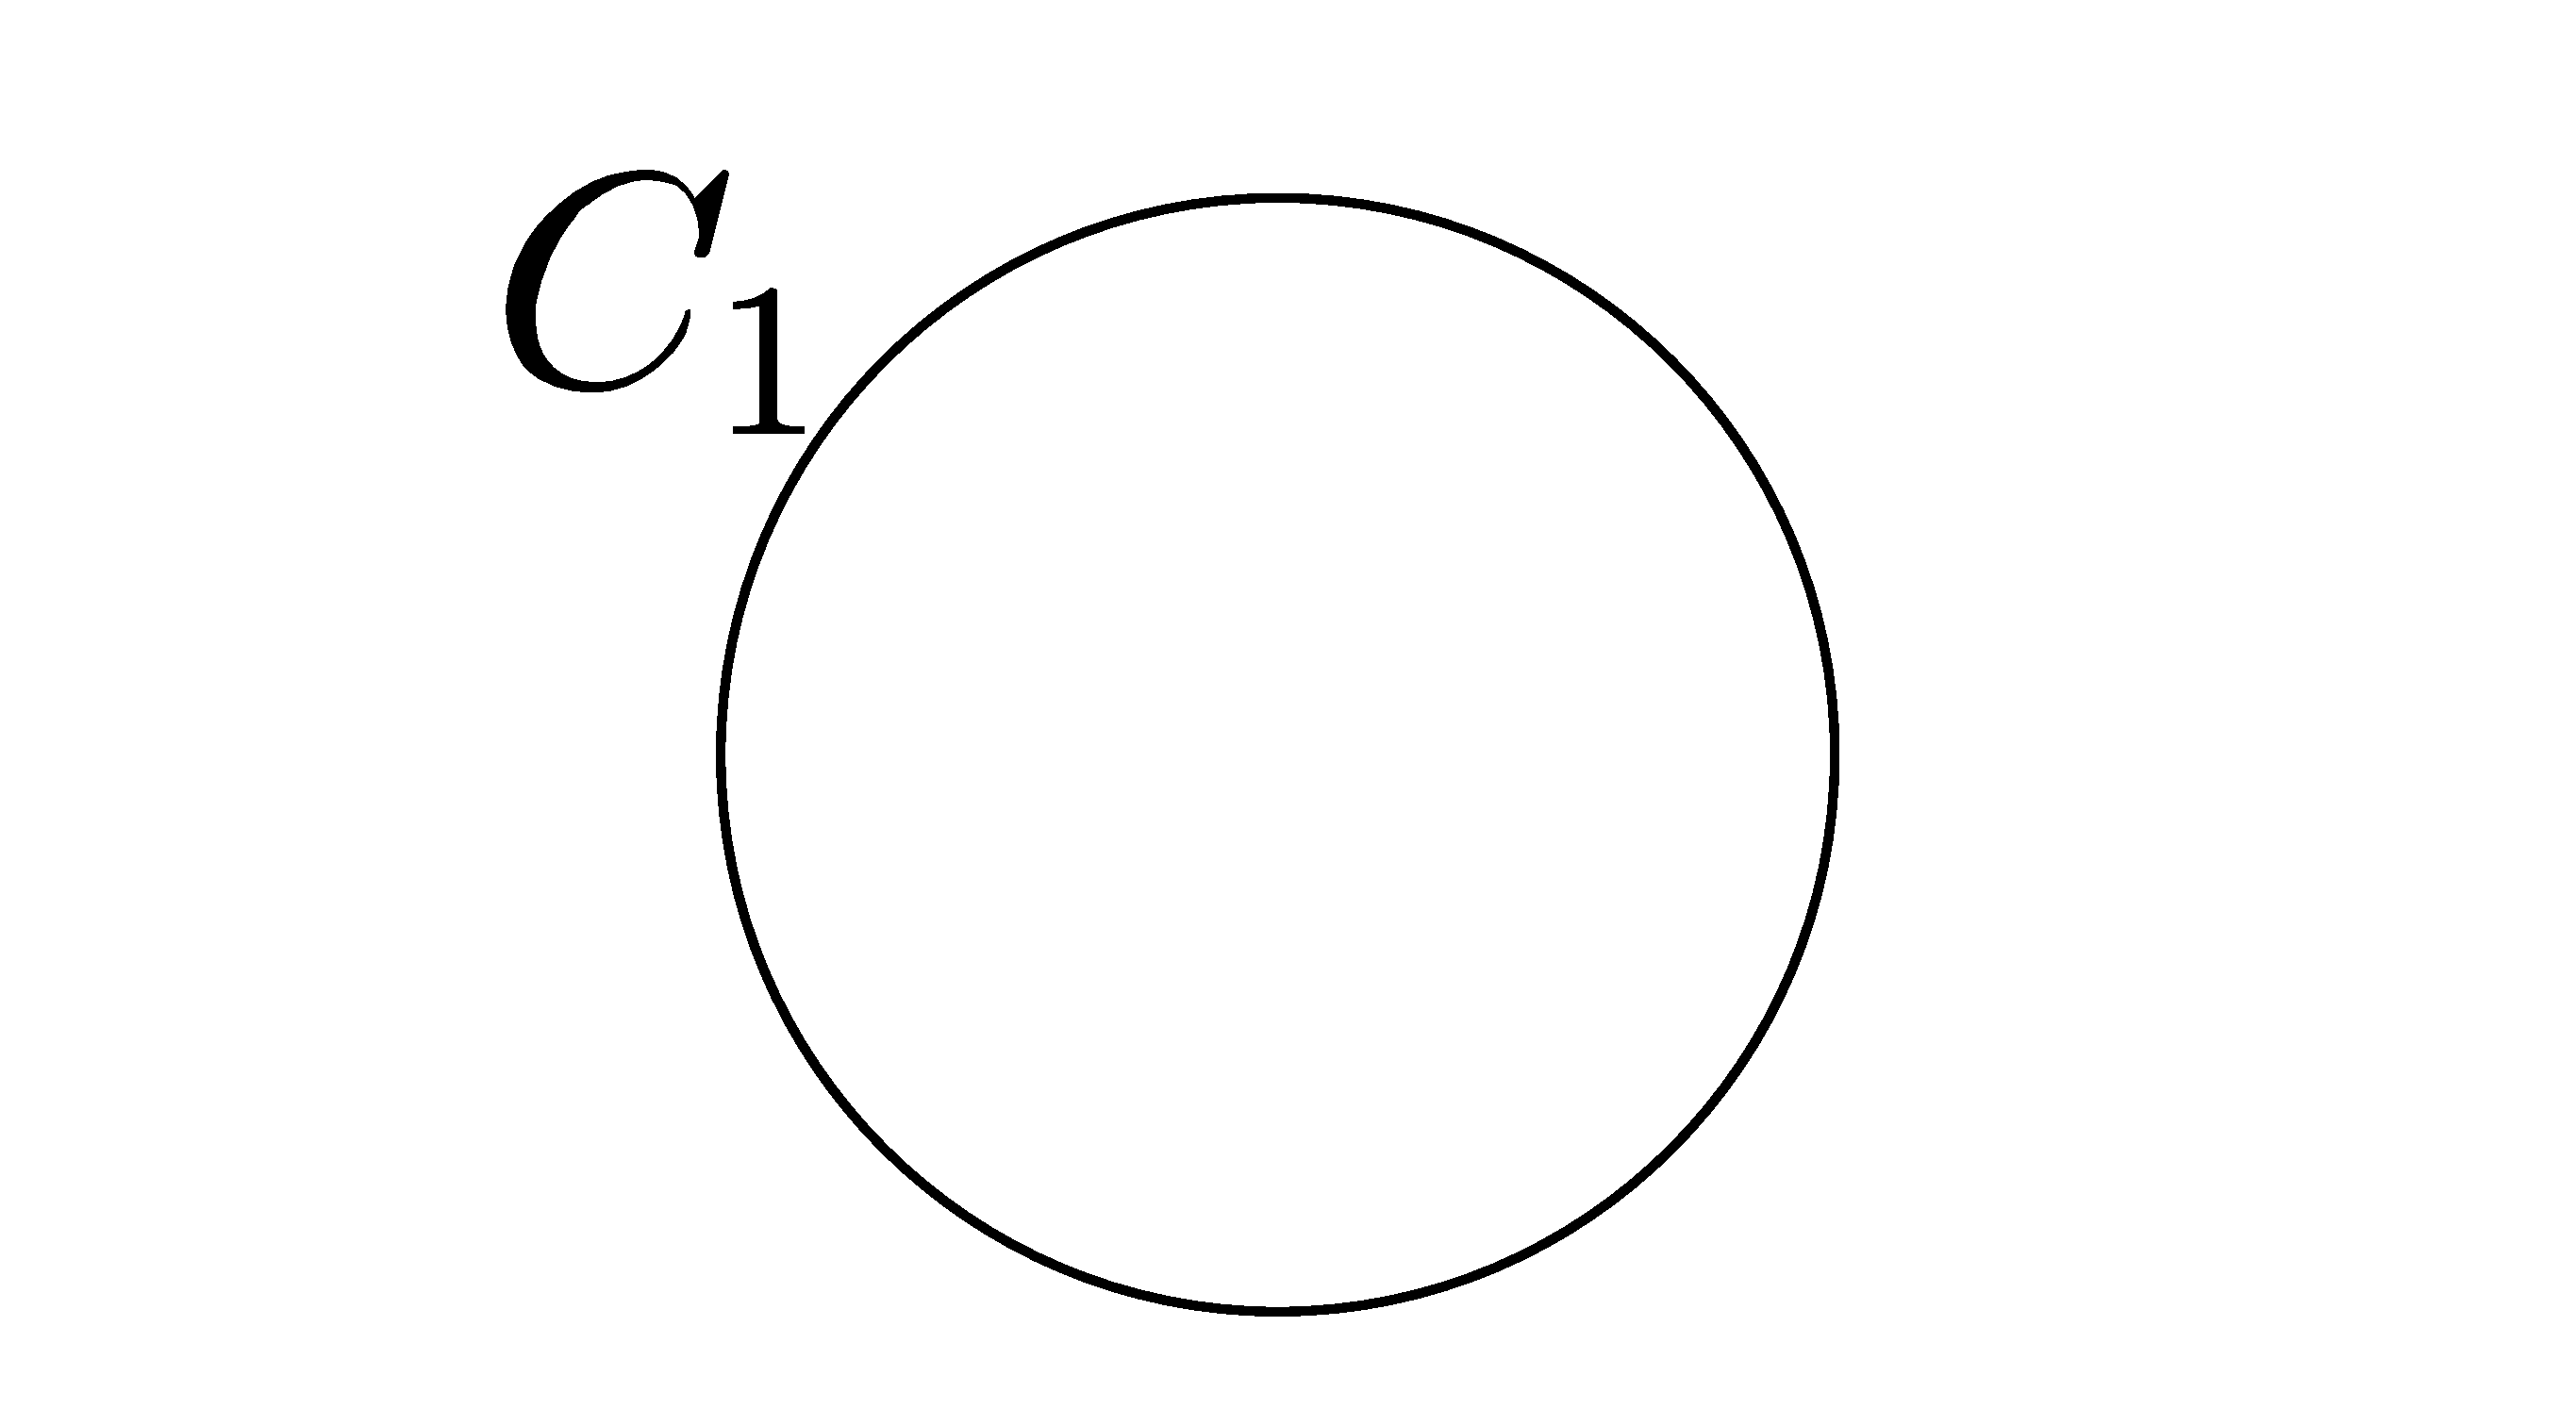
\includegraphics[scale=.065]{Graficos/elipse.eps}}
	\subfigure[Hipérbola]{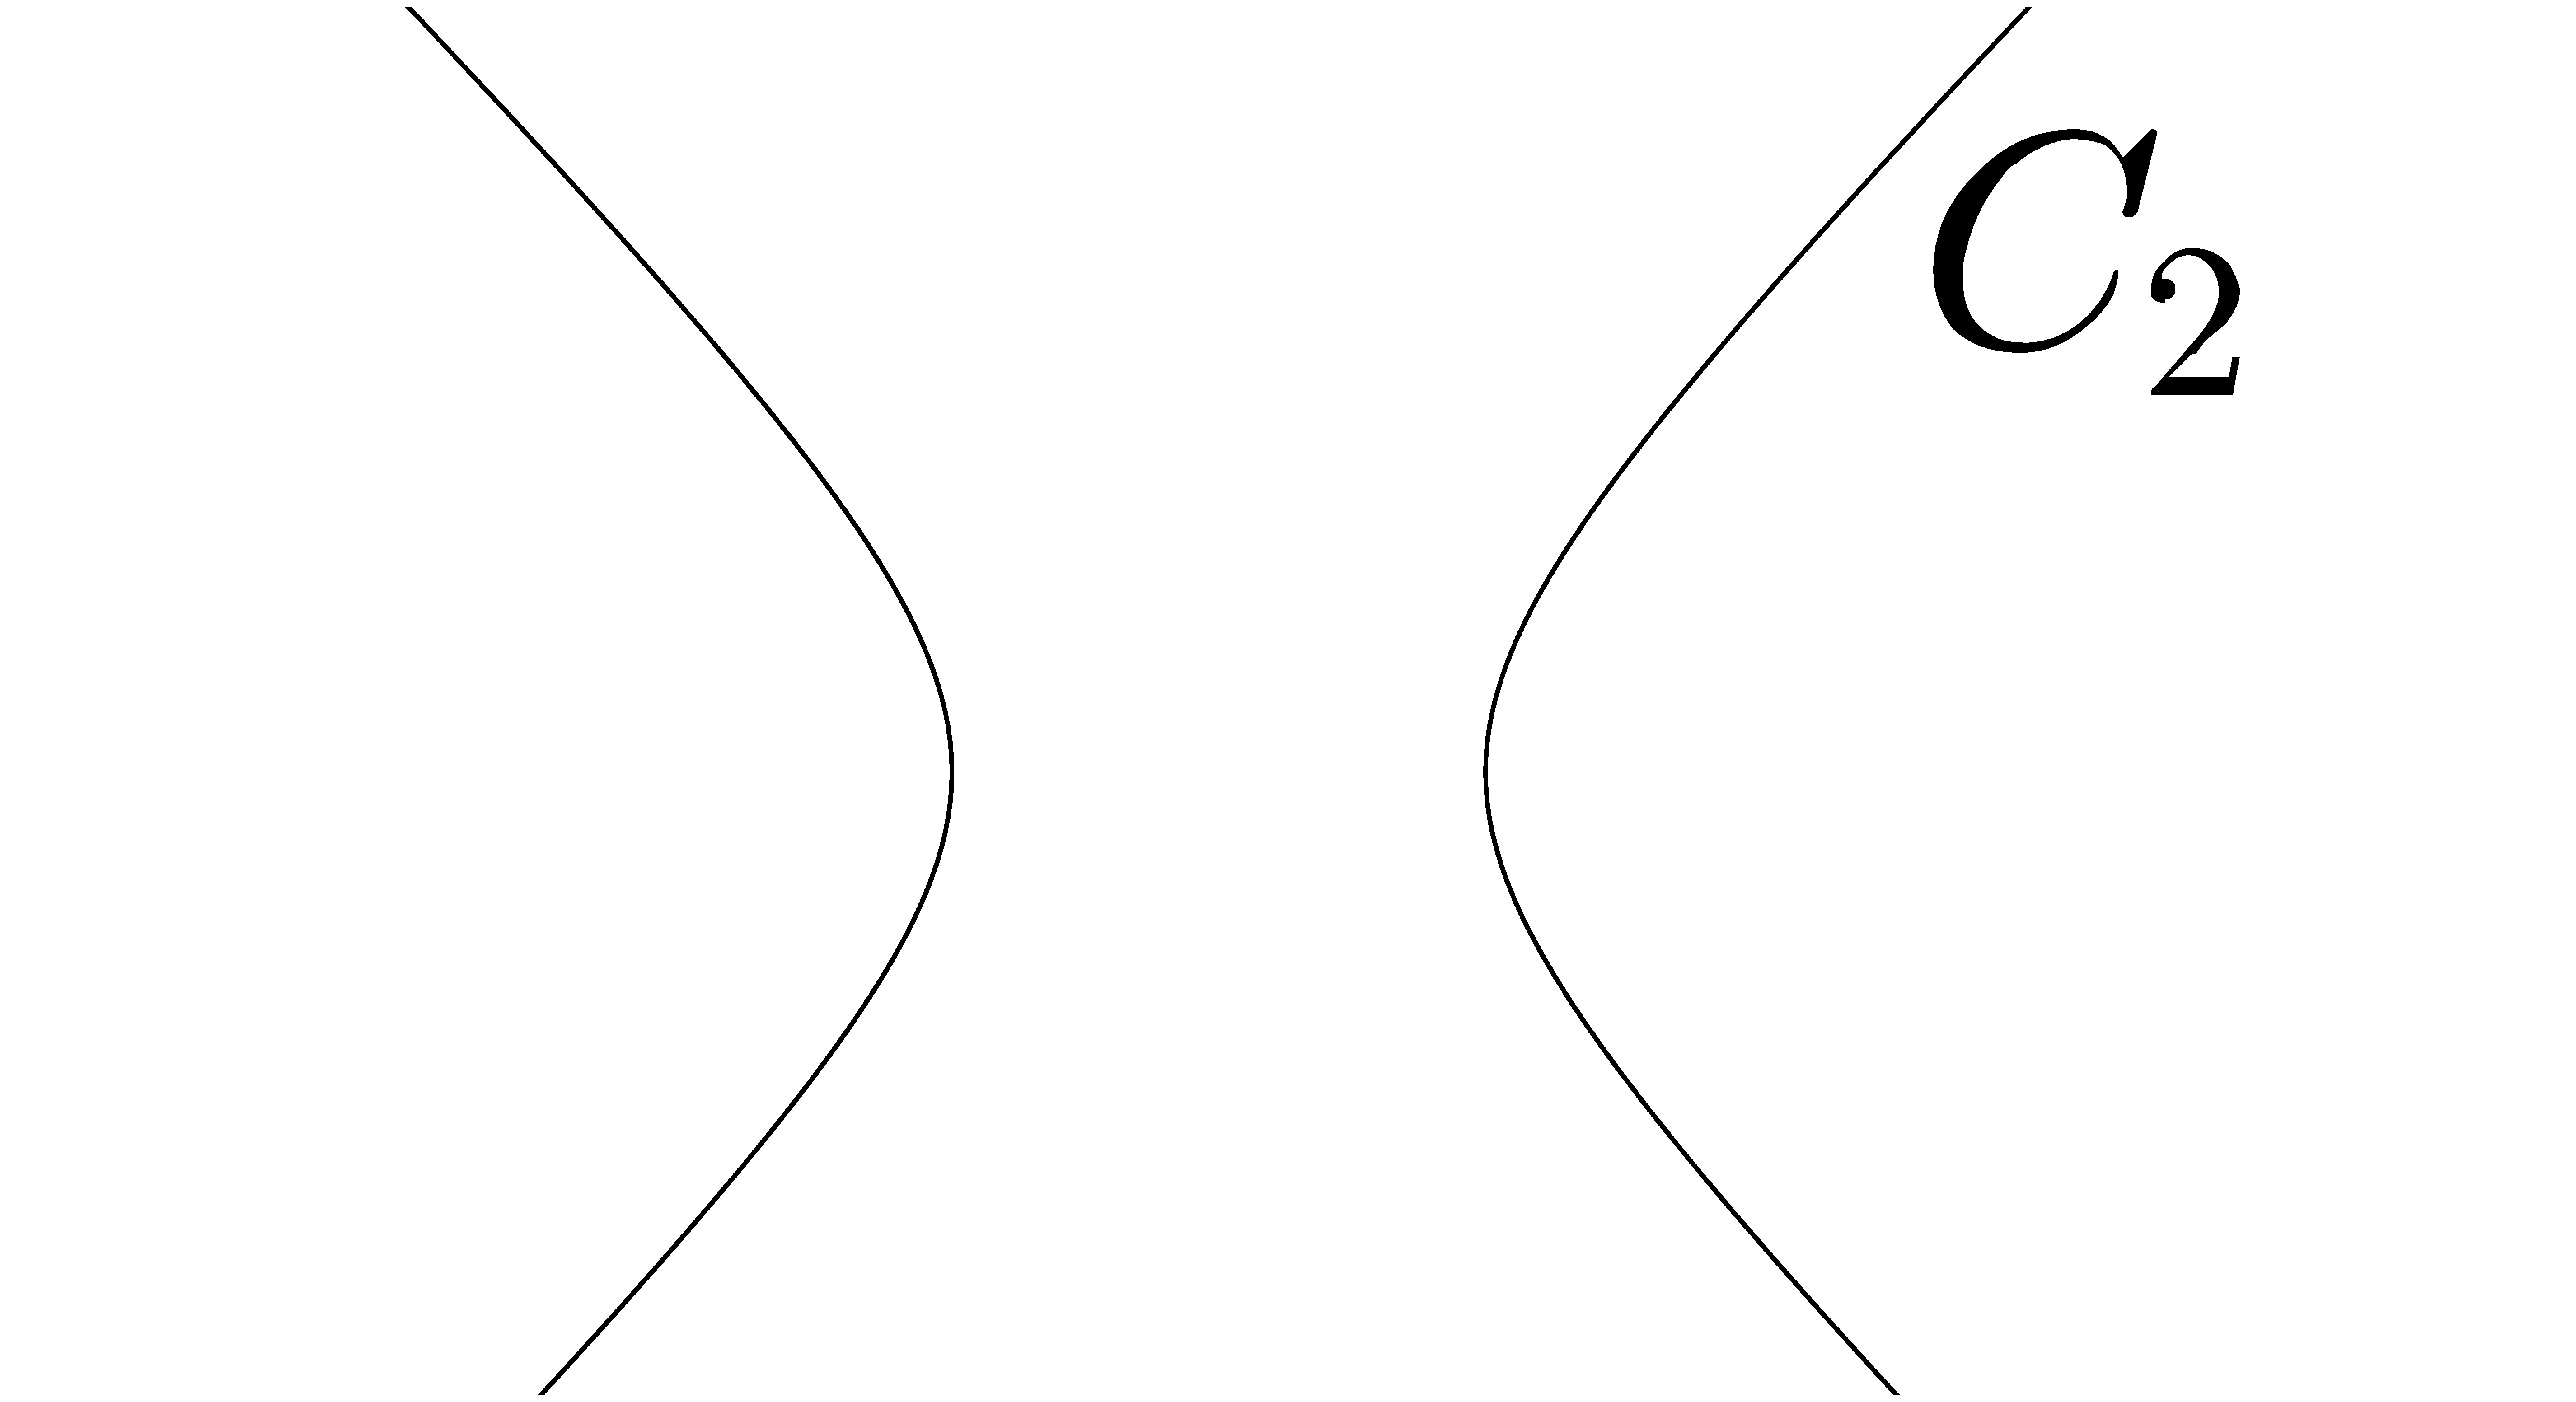
\includegraphics[scale=.028]{Graficos/hiperbola.eps}}
	\subfigure[Parábola]{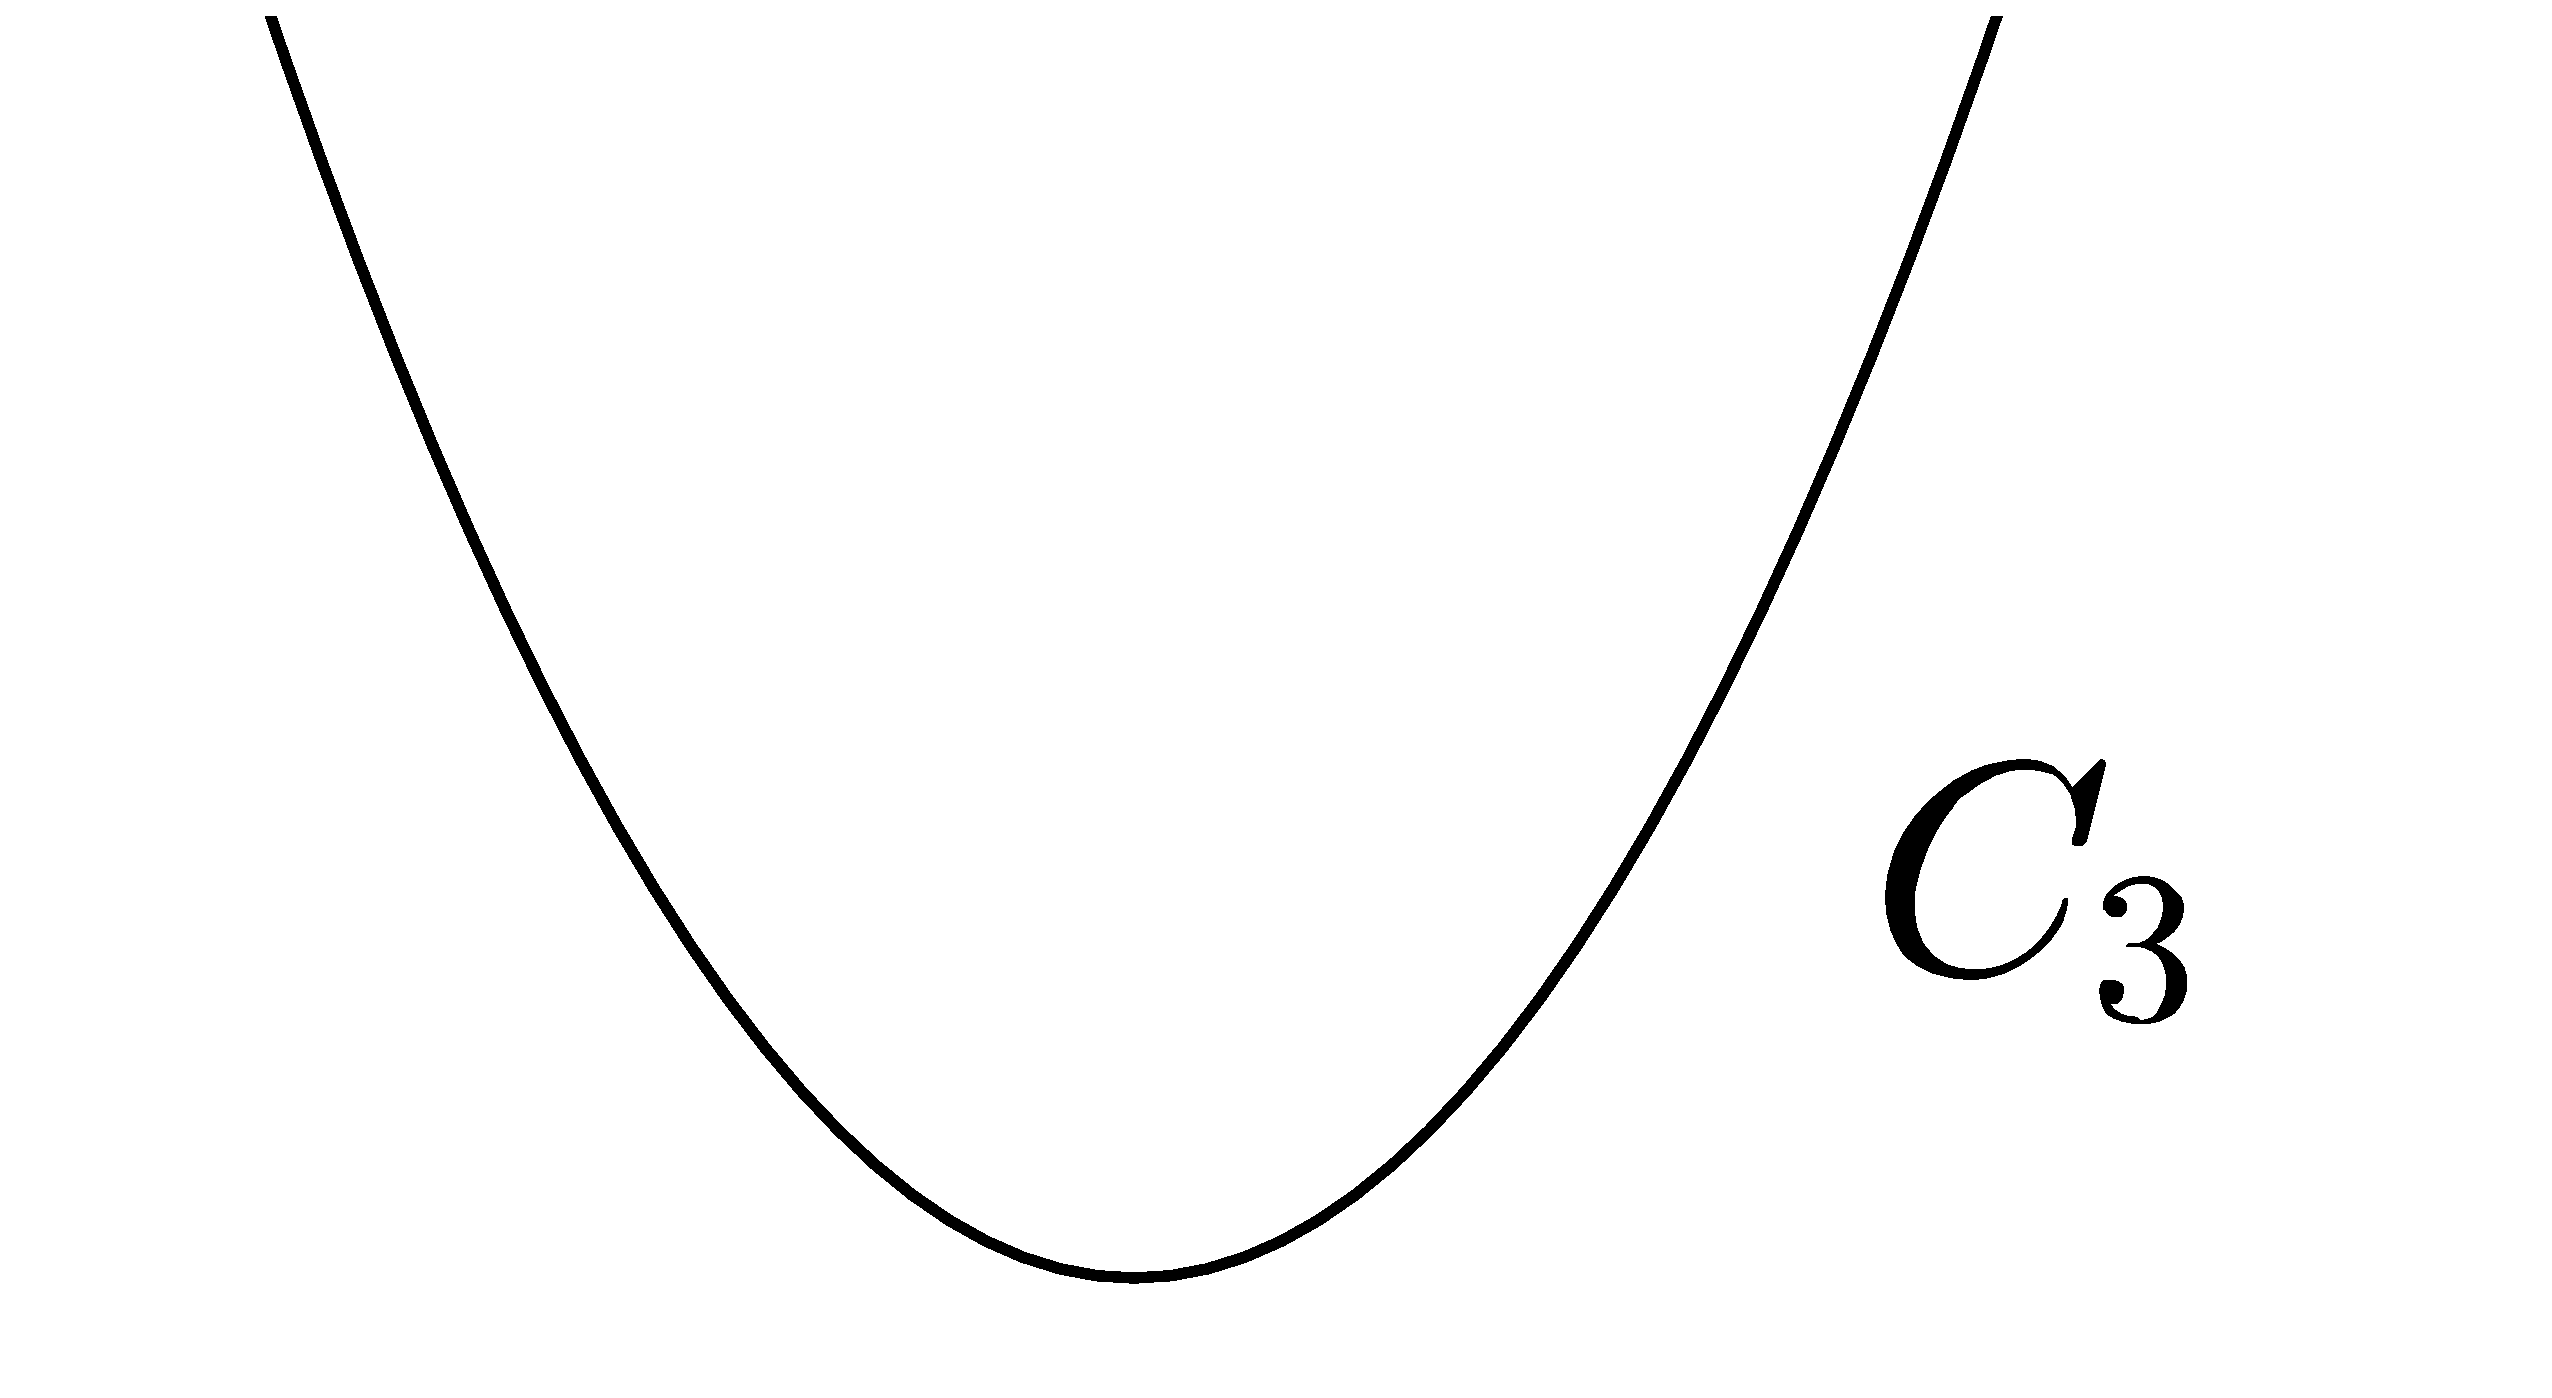
\includegraphics[scale=.06]{Graficos/parabola.eps}}
	\caption{Ilustración de los tipos de cónicas.}
	\label{C7_img_tiposConicas}
\end{figure}
Para que esta clasificación no resulte demasiado abstracta al lector, pongamos un ejemplos de cónicas de cada uno de los tipos.
\begin{exa}[Elipse]
	\label{C8_exa_elipse}
	Consideramos la cónica dada por la siguiente ecuación:
	\[C:x^2+y^2-z^2=0\]
	Intersequemos la cónica con la recta $l_\infty:z=0$ para poder clasificarla.
	\[\left.\begin{array}{c}
	x^2+y^2-z^2=0\\
	z=0
	\end{array}\right\}\leadsto x^2+y^2=0\]
	Es claro que la única solución a esta ecuación es el punto $(0,0,0)$, sin embargo, el rayo engendrado por este vector no está definido. Por ende, no hay ningún rayo (punto proyectivo) de la cónica que sea, a la vez, un rayo de la recta del infinito. Por ende, esta cónica es una elipse.
\end{exa}
\begin{exa}[Hipérbola]
	Clasifiquemos la cónica de ecuación:
	\[C:X^2-Y^2=1\]
	Antes de que cunda el pánico, nótese que esta ecuación nos viene dada en forma ``deshomogeneizada'' (si no no sería la ecuación de una cónica). Al homogeneizarla nos queda algo bastante más familiar:
	\[C:x^2-y^2-z^2=0\]
	Calculemos los puntos de corte con $z=0$:
	\[\left.\begin{array}{c}
	x^2-y^2-z^2=0\\
	z=0
	\end{array}\right\}\leadsto x^2=y^2\]
	Tomando raíces cuadradas y considerando todos los casos necesarios obtemos como soluciones los puntos de la forma:
	\[\begin{array}{cc}
	\class{(\lambda,\lambda,0)}=(1:1:0)\qquad & \qquad \class{(\lambda,-\lambda,0)}=(1:-1:0)
	\end{array}\]
	Por ende, la cónica $C$ tiene dos puntos de corte con la recta del infinito, esto significa que es de tipo hiperbólico.
\end{exa}
\begin{exa}[Parábola]
	Se nos da la siguiente cónica en forma no homogénea:
	\[C:Y=X^2\]
	Calculemos (tras homogeneizar) los puntos de corte de la misma con $l_\infty$.
	\[\left.\begin{array}{c}
	zy-x^2=0\\
	z=0
	\end{array}\right\}\leadsto x^2=0\]
	Teniendo en cuenta esto, los puntos que cumplen las restricciones impuestas por ambas ecuaciones son los de la forma $(0,\lambda,0)$ (los cuales, además, son solución doble). Estos generan un único rayo. Por ende, la cónica y la recta del infinito únicamente se cortan en un punto. Esto es lo mismo que decir que $C$ es una parábola.
\end{exa}
\section{Deshomogeneizaciones de una Cónica}

\section{Cuádricas, cónicas y cambio de referencia}
Hasta ahora hemos hablado de cuádricas y su matriz asociada en cierta referencia proyectiva. Pero ¿y si queremos escribir la ecuación de la cuádrica o su matriz en otra referencia? A continuación veremos como hacer esto.\\

Sean dos referencias proyectivas $\mf{R}$ y $\overline{\mf{R}}$ del espacio proyectivo $\proy^n$. El cambio de la referencia $\mf{R}$ a $\overline{\mf{R}}$ viene descrito por las siguientes ecuaciones
\begin{equation}
\rho X=M\overline{X}
\end{equation}
donde $M$ es la matriz de paso. 

Partimos de una cuádrica que en la referencia $\mf{R}$ tiene ecuaciones
\begin{equation}
X^tAX=0
\end{equation}
donde $A$ es la matriz de la cuádrica en esta referencia. Nuestro objetivo es escribir la cuádrica en la referencia $\overline{\mf{R}}$., es decir, buscamos la matriz $\overline{A}$ tal que
\begin{equation}
\overline{X}^t\overline{A}\overline{X}=0
\end{equation}
Para ello utilizamos las ecuaciones de cambio de referencia. Dado que la matriz de la cuádrica, y con ello su ecuación, es única salvo múltiplo, omitiremos el parámetro $\rho$ en los siguientes cálculos.
\begin{equation}
X^tAX=0\Leftrightarrow (M\overline{X})^tA(M\overline{X})=0\Leftrightarrow \overline{X}^t M^tAM\overline{X}=0
\end{equation}
Se concluye pues que la matriz de la cuádrica en la referencia $\overline{\mf{R}}$ es $M^tAM$. Por tanto, las ecuaciones que relacionan la matriz de la cuádrica en la referencia ${\mf{R}}$ con su matriz en la referencia $\overline{\mf{R}}$ son
\begin{equation}
\label{C8_eq_relacionMatrices_referencias}
\rho\overline{A}=M^tAM
\end{equation}
donde $M$ recordemos que es la matriz de cambio de referencia. Se observa que, si $A$ es simétrica, entonces $\overline{A}$ seguirá siendo simétrica. En efecto
\begin{equation}
(\rho\overline{A})^t=(M^tAM)^t=M^tA^tM=M^tAM=\rho\overline{A}
\end{equation}
Gracias a esto hallar los coeficientes de la matriz $\overline{A}$ pasa a ser una tarea sencilla. Particularicemos por un momento al caso en el que nos encontramos en $\proy^2$ para ver el gran cambio que esto supone.

Si $\overline{A}$ no fuese una matriz simétrica, al ser una matriz $3\times 3$, tendríamos $9$ parámetro a determinar, que se transformarían en $8$ si consideramos la proyección del espacio vectorial de las matrices $3\times 3$, es decir, si nos da igual considerar $\overline{A}$ o $\lambda\overline{A}$. En cambio, al ser simétrica estos se reducen a $5$, ya que, como vimos en la observación~\ref{C8_obs_conica_p5} , $\proy(\mathrm{Sim}(3))$ es isomorfo a $\proy^5$. Esto supone una gran diferencia frente a los $9$ parámetros iniciales. 

Recordemos, del ejemplo~\ref{C8_exa_coordenadas_conica_p5}, que, a su vez, estos coeficientes de la matriz $\overline{A}$ son las coordenadas de la cónica en $\proy^5$, con lo cual la cónica queda perfectamente determinada.\\

Este tipo de trasformaciones preservan el rango de la matriz. Esto se debe a que $A$ y $\overline{A}$ son congruentes, es decir, que existe una matriz $P$ tal que $\overline{A}=P^tAP$. Por tanto, en particular, son equivalentes.

Esto implica que, si partimos de una cónica no degenerada con matriz $A$ es imposible que al hacer un cambio en el sistema de referencia proyectivo obtengamos una matriz degenerada, pues $rg(A)=rg(\overline{A})$. Sin embargo, cabe esperar que mediante un cambio de referencia se pueda trasformar una cónica en cualquier otra (preservando la degeneración), como veremos más adelante.

\section{Cónicas degeneradas}
\label{C8_sec_conicas_degeneradas}
Al igual que hicimos con cónicas no degeneradas, realizaremos una clasificación de cónicas degeneradas. Aunque esta clasificación terminará siendo mucho más simple que la que tenemos para cónicas no degeneradas, llegar a ella conlleva más trabajo. Por ello, iremos desarrollando una serie de lemas y proposiciones que nos guiarán al resultado final. Comenzamos definiendo una cónica degenerada.
\begin{defi}
	Diremos que una cónica, dada por la ecuación
	\begin{equation}
	C:X^tAX=0
	\end{equation}
	es \ti{degenerada} si contiene una recta.
\end{defi}

Esta definición de cónica degenerada no es muy manejable. Por ello, veamos la siguiente proposición
\begin{prop}\label{C8:prop_rango_menor_3_degenerada}
	Sea $C$ una cónica cuya matriz en cierta referencia es $A$. Si $rg(A)<3$ entonces $C$ es una cónica degenerada.
\end{prop}

\begin{proof}
	Para demostrar que la cónica $C$ es degenerada veamos que contiene una recta. Si el rango de la matriz $A$ es menor que $3$, entonces el núcleo de $A$ no es vacío. Por tanto, existe un vector $y_0$ tal que $AY_0=0$, donde $Y_0$ representa el vector columna de $y_0$. Esto implica que $Y_0^tAY_0=0$, por lo que, al menos, el punto $[y_0]$ pertenece a la cónica.
	
	Sea $[z_0]$ otro punto de la cónica, distinto de $[y_0]$. Veamos que la recta $YZ$ generada por $[z_0]$ e $[y_0]$ está contenida en la cónica. Con esto quedaría demostrado que la cónica es degenerada.
	
	Sea un punto $[y_0+\theta z_0]$ de la recta $YZ$. Si este punto perteneciese a $C$ para todo $\theta$, la recta $YZ$ estaría contenida en la cónica. Veamos que cumple la ecuación de la cónica, sea cual sea el valor de $\theta$:
	\begin{equation}\label{C8:eq_joanch_conicas_deg}
	(Y_0+\theta Z_0)^tA(Y_0+\theta Z_0)=Y_0^tAY_0+\theta Y_0^tAZ_0+\theta Z_0^tAY_0+\theta^2Z_0^tAZ_0=Y_0^tAY_0+2\theta Z_0^tAY_0+\theta^2Z_0^tAZ_0
	\end{equation}
	El primer y segundo sumando se anulan debido a que $y_0$ pertenece al núcleo de $A$. El tercero por su parte se anula porque $\class{z_0}$ pertenece a la cónica. De esto se concluye que
	\begin{equation}
	(Y_0+\theta Z_0)^tA(Y_0+\theta Z_0)=0 \quad \forall\theta
	\end{equation}
	finalizando así la demostración.
\end{proof}

A continuación veamos un teorema que nos da la expresión de una cónica degenerada.

\begin{theo}\label{C8:theo_conica_degenerada_es_producto_rectas}
	Una cónica $C$ es degenerada si y solo si es producto de dos rectas. Es decir, es de la forma
	\begin{equation}
	C:l\cdot m=0 \quad o \quad C:l^2=0
	\end{equation}
	donde $l$ y $m$ son rectas distintas.
\end{theo}

\begin{proof}
	$\bla$ Esta implicación quedó demostrada en la observación~\ref{C8_obs_conicaProducto_union}. En ella se vio que, si una cónica es producto de dos rectas (iguales o distintas), entonces contiene una recta, siendo, por tanto, una cónica degenerada.
	
	$\bra$ Sea la cónica $C$ descrita por la ecuación
	\begin{equation}\label{eq_conica_teo_degenerada}
	C: ax^2+by^2+cz^2+2fyz+2gxz+2hxy=0
	\end{equation}
	Si es degenerada entonces, por definición, contiene una recta $l$. Cambiando de referencia, si es preciso, podemos suponer que la recta es $l:x=0$. Dado que la recta está contenida en la cónica, la ecuación~\eqref{eq_conica_teo_degenerada} debe anularse en todos los puntos de la recta, es decir, en todos los puntos de la forma $(0,y,z)$ cualesquiera que sean $z$ e $y$. Con ello
	\begin{equation}
	by^2+cz^2+2fyz=0 \quad \forall y,z \Leftrightarrow b=c=f=0
	\end{equation}
	La cónica pasa a ser
	\begin{equation}
	C: ax^2+2gxz+2hxy=x(ax+2gz+2hy)=0
	\end{equation}
	donde $ax+2gz+2hy=0$ es la ecuación implícita de una recta. Se obtiene así que $C:l\cdot m=0$ donde $m$ puede ser igual o distinta a $l$.
\end{proof}

Una vez demostrado este teorema podemos hacer una clasificación de las cónicas degeneradas atendiendo al rango de $A$. Para ello demostremos primero el siguiente lema.

\begin{lem}\label{C8:lem_nucleo_interseccion_rectas}
	Sea $C:l\cdot m=0$ una cónica degenerada con matriz $A$ simétrica. Entonces, el núcleo de $A$ es la intersección de las rectas $l$ y $m$.
\end{lem}

\begin{proof}
	Veamos primero que $l\cap m\subset \ker(A)$. 
	
	Sean las rectas $l$ y $m$ con ecuaciones implícitas
	\begin{equation}
	l:u^tX=0\ , \quad m:v^tX=0
	\end{equation}
	Ya vimos que podíamos escribir la cónica como
	\begin{equation}
	l\cdot m=X^t(uv^t+vu^t)X=0
	\end{equation}
	donde la matriz de la cónica $A=uv^t+vu^t$ es simétrica. Sea un punto $[y_0]$ perteneciente a la intersección de ambas rectas. Entonces cumple sus ecuaciones, es decir,
	\begin{equation}
	l:u^tY_0=0\ , \quad m:v^tY_0=0
	\end{equation}
	Por tanto,
	\begin{equation}
	AY_0=(uv^t+vu^t)Y_0=uv^tY_0+vu^tY_0=0
	\end{equation}
	con lo que $y_0\in \ker(A)$.\\
	
	Veamos que $\ker(A)\subset l\cap m$. Sea un punto del núcleo $[y_0]\in \ker(A)$. Por lo visto en la demostración de la proposición~\ref{C8:prop_rango_menor_3_degenerada} se tiene que, dado un punto cualquiera $[z_0]$ de la cónica distinto de $[y_0]$, la recta generada por ambos puntos está contenida en la cónica. Si la cónica es producto de dos rectas iguales ya hemos terminado, pues esa recta es precisamente la engendrada por $[z_0]$ e $[y_0]$. Sino, puedo coger otro punto $[w_0]$ de la cónica, que no pertenezca a la recta generada por $[z_0]$ e $[y_0]$. De nuevo, la recta generada por $[w_0]$ e $[y_0]$ está contenida en la cónica. Por tanto, $[y_0]$ pertenece a las dos rectas de la cónica, es decir, está en la intersección.
\end{proof}
Este lema, junto con el teorema anterior, nos permiten clasificar las cónicas degeneradas. 

Sabemos que una cónica degenerada es producto de dos rectas distintas o de dos iguales. Si el rango de la matriz asociada es $rg(A)=2$ entonces el $\ker(A)$ es un único punto. Esto implica, por el lema anterior, que las rectas intersecan en un punto, por lo que se trata de una cónica producto de dos rectas distintas. Por otro lado, si $rg(A)=1$ entonces el $\ker(A)$ es una recta. Atendiendo de nuevo al lema anterior, de esto se deduce que la cónica es producto de dos rectas iguales.

Todas estas deducciones pueden hacerse en sentido inverso aplicando el lema~\ref{C8:lem_nucleo_interseccion_rectas}. Sin embargo, recordemos que esto ya había sido demostrado, a través de otro razonamiento, en el apartado ''Rango de la Matriz de una Cónica producto de Rectas" de la sección~\ref{C8_subsec_producto_rectas}. Como prometimos, aquí está la otra implicación.

Resumiendo, sea una cónica degenerada $C:l\cdot m=0$, entonces
\begin{equation}
\begin{split}
l\not=m &\Leftrightarrow rg(A)=2,\\
l=m&\Leftrightarrow rg(A)=1.
\end{split}
\end{equation}

Veamos un ejemplo de como hallar la expresión de una cónica degenerada.

\begin{exa}
	Sea la cónica degenerada
	\begin{equation}
	C: x^2-y^2-xz+yz=0
	\end{equation}
	Expresar la cónica como producto de dos rectas.
	
	La matriz de la cónica es
	\begin{equation}
	A=\left( \begin{array}{rrr}
	1&0&-\frac{1}{2}\\
	0&-1&\frac{1}{2}\\
	-\frac{1}{2}&\frac{1}{2}& 0
	\end{array}\right) \sim
	\left( \begin{array}{rrr}
	2&0&-1\\
	0&-2&1\\
	-1&1&0
	\end{array}\right)
	\end{equation}
	Se trata de hacer con una cónica concreta lo explicado en la demostración del lema~\ref{C8:lem_nucleo_interseccion_rectas}. Si el núcleo de la matriz $A$ de la cónica es una recta, entonces la cónica es de la forma $l^2=0$ y la recta del núcleo es precisamente la recta $l$. Sino, como ocurre en este caso, dado un punto del núcleo de $A$, la recta generada por él y por otro punto distinto de la cónica está contenida en ella. Por tanto, si hallamos dos puntos pertenecientes a la cónica, distintos entre ellos y al núcleo de la matriz, podremos generar dos rectas distintas, que serán las rectas de $C$.
	
	Buscamos pues el núcleo de la matriz $A$.
	\begin{equation}
	A\left( \begin{array}{c}
	x\\y\\z
	\end{array}\right) =\left( \begin{array}{c}
	0\\0\\0
	\end{array}\right)\Leftrightarrow
	\begin{cases}
	2x-z=0\\
	-2y+z=0\\
	-x+y=0
	\end{cases}
	\end{equation}
	Por tanto, el núcleo de $A$ es el punto $y_0=(x:y:2x)=(1:1:2)$. Lo más fácil para conseguir dos puntos de la cónica $C$ distintos entre ellos y a $y_0$ es intersecar la cónica con una recta, que no contenga a $y_0$. En este caso, por ejemplo, elegimos la recta $z=0$. La intersección viene dada por:
	\begin{equation}
	\begin{cases}
	x^2-y^2-xz+yz=0\\
	z=0
	\end{cases}\Leftrightarrow x^2+y^2=0\Leftrightarrow (x-y)(x+y)=0\Leftrightarrow x=y, \ x=-y
	\end{equation}
	Por tanto, los puntos de la intersección son $z_0=(x:x:0)=(1:1:0)$ y $w_0=(x:-x:0)=(1:-1:0)$. Finalmente, las rectas de la cónica son las generadas por $y_0$ y $z_0$ y por $y_0$ y $w_0$. Sus ecuaciones implícitas son:
	\begin{equation}
	\begin{split}
	y_0z_0&:x-y=0\\
	y_0w_0&:x+y-z=0
	\end{split}
	\end{equation}
	Por tanto, la cónica $C$ es
	\begin{equation}
	C: (x-y)(x+y-z)=0
	\end{equation}
\end{exa}
Cualquiera diría que este es el procedimiento habitual para hallar la expresión de una cónica degenerada como producto de rectas. Desde luego, no lo es. Más adelante veremos como hacer esto decentemente.
\begin{obs}
	La intersección entre una cónica y una recta viene dada por una ecuación de segundo grado, que tendrá dos soluciones (bien sean distintas o dobles). Por tanto, siempre nos es posible encontrar una recta que corte en dos puntos con la cónica.
	
	En efecto, una recta viene parametrizada por dos puntos $y_0$ y $z_0$ de la forma $[y_0+\theta z_0]$. La intersección de esta recta con la cónica serán aquellos puntos, es decir aquellos valores de $\theta$, para los que el vector columna $Y_0+\theta Z_0$ cumple la ecuación de la cónica. La ecuación resultante de sustituir dicho vector en la ecuación de la cónica es la mostrada en la ecuación~\eqref{C8:eq_joanch_conicas_deg}, que es de segundo grado en la variable $\theta$. Más adelante daremos nombre a esta ecuación.
\end{obs}

\section{Recta polar de un punto respecto de una cónica}
Volvamos a las cónicas no degeneradas para tratar un concepto de gran utilidad, y que posteriormente trasladaremos a cónicas degeneradas.

Comenzaremos definiendo recta polar. Sin embargo, esta definición no nos permite hacernos una idea de cuál es exactamente esta recta. Por ello presentamos antes la siguiente construcción geométrica que, sin ser la definición de recta polar, nos permite ver que recta es. Además, veremos que, si construimos la recta polar a partir de la definición, obtenemos la recta indicada en la figura.

IMAGEN

\begin{defi}
	Sea una cónica, un punto $P$ y $r$ una recta perteneciente al haz de base $P$. Sean $M$ y $N$ los puntos de corte de la recta $r$ con la cónica. Se define \ti{recta polar del punto $P$} al conjunto de puntos $P'$ que son el cuarto armónico de $P$ respecto al par $(M,N)$, y que se obtienen al variar $r$.
\end{defi}
\begin{defi}
	Sea una recta $r$ la recta polar de un punto $P$, entonces $P$ es el \ti{polo} de $r$.
\end{defi}

La recta polar del punto $P$ respecto a una cónica se denota Polar($P$). Equivalentemente, se podría decir que la recta Polar(P) está formada por los puntos $P'$ tales que el par $(P,P')$ separa armónicamente al par $(M,N)$, donde $M$ y $N$ varían con $r$.\\

A partir de la definición determinemos la ecuación implícita de la recta polar de un punto $P$. Aunque la definición es válida para cualquier punto $P$, ya esté en la cónica, sea exterior a ella o interior, comenzaremos tomando un punto $P$ que se encuentre fuera de la cónica. 

Así pues, sea $C$ una cónica, cuya ecuación viene dada por
\begin{equation}
X^tAX=0,
\end{equation}
y un punto $P$ exterior a $C$. Sea una recta arbitraria $r$ del haz de base $P$ tal que $r\cap C=\{M,N\}$, con $M$ y $N$ distintos. Buscamos los puntos $P'$ tales que $\{M,N;P,P'\}=-1$. Por tanto, $P'$ debe estar en la recta $r$. Parametrizamos la recta $r$, tomando representantes de los puntos $P=[\vec{p}]$ y $P'=[\vec{p}']$:
\begin{equation*}
	r:[\vec{p}+\theta \vec{p}']
\end{equation*}
De esta forma podemos escribir
\begin{equation*}
	M=[\vec{p}+\theta_M \vec{p}'] \ , \quad N=[\vec{p}+\theta_N \vec{p}'] \ , \quad P=0 \ , \quad P'=\infty \ ,
\end{equation*}
donde $\theta_M$ y $\theta_N$ son las coordenadas no homogéneas de los puntos de corte $M$ y $N$, y $P$ y $P'$ se expresan en coordenadas no homogéneas.

Por tanto, 
\begin{equation}
-1=\{M,N;P,P'\}=\{\theta_M,\theta_N;0,\infty\}\Leftrightarrow \theta_M=-\theta_N
\end{equation}
Tenemos así una restricción para los puntos $M$ y $N$. Recordemos que además son la intersección de la recta $r$ con la cónica $C$. Los puntos de corte viene dados por la ecuación
\begin{equation}
(\vec{P}^t+\theta \vec{P}')^tA(\vec{P}^t+\theta \vec{P}')=\vec{P}^tA\vec{P}+2\theta \vec{P}^tA\vec{P}'+\theta^2\vec{P}'^tA\vec{P}'=0
\end{equation}
que se obtiene simplemente de sustituir la ecuación paramétrica de $r$, donde $\vec{P}$ son vectores columna, en la ecuación de la cónica (cosa que ya hemos hecho antes varias veces). Recibe el nombre de \textbf{ecuación de Joachimstal} y nos permite calcular la intersección de una cónica y una recta.

Dado que en este caso la intersección son los puntos $M$ y $N$, las soluciones a esta ecuación deben ser $\theta_N$ y $\theta_M=-\theta_N$. Una ecuación de segundo grado tiene soluciones iguales y de signo opuesto si y solo si el término de grado uno es nulo. Por tanto, necesariamente
\begin{equation}\label{C8:eq_puntos_recta_polar}
\vec{P}^tA\vec{P}'=0
\end{equation}
Por ende, los puntos $P'$ buscados deben cumplir esta ecuación.

El punto $P$ y la matriz $A$ son conocidos, por tanto, el producto $\vec{P}^tA$ dará como resultado el vector $u=(u_1, u_2,u_3)$ conocido. El punto $P'$ es desconocido, pudiéndolo escribir como $(x, y,z)$. De esta forma, los puntos $P'$ de la recta Polar(P) deben cumplir
\begin{equation}
(u_1 \ u_2 \ u_3)
\left( \begin{array}{c}
x\\ y\\ z
\end{array}\right) =0
\end{equation}
Notemos que esto es la ecuación de una recta con coeficientes $u_1,u_2$ y $u_3$. Dado que los puntos que cumplen la ecuación son los $P'$, esta no es otra que la ecuación implícita de la recta polar del punto $P$ respecto a la cónica $C$.

Es decir, los coeficientes de la recta Polar(P) vienen dados por
\begin{equation}
u=\vec{P}^tA\Rightarrow u^t=A\vec{P}
\end{equation}
Si el punto $P$ fuese interior a la cónica, los puntos de corte de las rectas del haz con base $P$ y la cónica $C$ serían puntos imaginarios conjugados.
\begin{obs}
	Conviene recordar la notación utilizada en este apartado, pues será usada en ocasiones de aquí en adelante. En concreto, $P$ es un punto proyectivo tal que $P=[\vec{p}]$ y $\vec{P}$ es el vector columna de $\vec{p}$.
\end{obs}

\begin{obs}
	El punto $P'$ pertenece a la recta polar de $P\Leftrightarrow  \vec{P}^tA\vec{P}'=0\Leftrightarrow \vec{P}'^tA\vec{P}=0\Leftrightarrow $ el punto $P$ pertenece a la recta polar de $P'$.
\end{obs}

Por tanto, dada una cónica, un punto $P$ exterior a la cónica y un punto $P'$ perteneciente a la recta Polar(P), si trazamos una recta que pasa por $P'$ y que corta a la cónica en dos puntos $M$ y $N$ y encontramos el cuarto armónico $Q$ de $P'$ respecto a $(M,N)$, la recta polar de $P'$ será aquella que pase por $Q$ y $P$ (pues al pertenecer $P'$ a la recta polar de $P$, $P$ pertenece a la recta polar de $P'$). Observamos que se encuentra fuera de la cónica. Esto es coherente con que los puntos de corte de Polar(P') con la cónica sean imaginarios, ya que $P'$ es un punto interior a la cónica.

IMAGEN

Hagamos ahora una construcción geométrica de la recta Polar(P) (mostrada en la figura ?). Para poder trazar esta recta debemos encontrar dos puntos que pertenezcan a ella, es decir, dos cuartos armónicos.

IMAGEN

Tomamos dos rectas $r_0$ y $r_1$ del Haz(P) que cortan con la cónica en los puntos $M_0$, $N_0$ y $M_1$, $N_1$, respectivamente. El cuarto armónico $P_0'$ de $P$ respecto del par $(M_0,N_0)$ pertenece a la recta Polar(P), al igual que el cuarto armónico $P_1'$ de $P$ respecto del par $(M_1,N_1)$. Tenemos así dos puntos que pertenecen a la recta polar del punto $P$.

Para encontrar los puntos $P_0'$ y $P_1'$ procedemos de la siguiente manera. Se recomienda ir dibujándolo mientras se explica para entender el proceso. Si se siguen los pasos indicados, la figura resultante debe ser equivalente a la figura ?.

Trazamos la recta que pasa por $N_0$ y $M_1$ y la que pasa por $N_1$ y $M_0$, las cuales se cortan en un punto $E$. De la misma forma, la recta que pasa por $N_0$ y $N_1$ y la que pasa por $M_0$ y $M_1$ se cortan en un punto $Q$. Finalmente, la recta que pasa por $Q$ y por $E$ es la recta Polar(P), que corta con $r_0$ y $r_1$ en los puntos $P_0'$ y $P_1'$.

Podríamos preguntarnos por qué la recta $QE$ es la recta polar, ya que lo hemos asegurado sin explicar nada. Obsérvese que lo único que hemos hecho ha sido la construcción geométrica de un cuadrilátero completo para los puntos $P,M_0,N_0$ y el punto de corte de $QE$ con $r_0$ ($P_0'$), y otro para los puntos $P,M_1,N_1$ y el punto de corte de $QE$ con $r_1$ ($P_1'$). Esto asegura que los puntos están separados armónicamente. Por tanto, necesariamente, la recta $QE$ es la recta polar, pues los puntos que pertenecen a ella son los $P'_i$ tales que $(P,P'_i)$ están separados armónicamente de $(M_i,N_i)$.\\

Al principio de esta sección se mostró una construcción geométrica y en ella se indicó la recta polar de un punto $P$. Para ver que, efectivamente, esa es la recta polar es necesario avanzar un poco más. Con ese fin, damos la siguiente definición.

\begin{defi}
	Una recta es \ti{tangente} a una cónica si la corta en un punto con multiplicidad mayor que uno.
\end{defi}
\begin{lem}
	Sea $r$ la recta polar de un punto $P$ respecto a una cónica $C$, con matriz $A$. Entonces, las rectas $PP_i'$ con $i=0,1$, donde $P_i'$ son los puntos de corte de la recta polar con la cónica, son tangentes a $C$.
\end{lem}
\begin{proof}
	La recta $PP_0'$ tiene como ecuación paramétrica
	\begin{equation*}
		[\vec{p}+\theta\vec{p_0}']
	\end{equation*}
	Para ver que es tangente a la cónica debemos comprobar que $P_0'$ es un punto de corte de multiplicidad mayor que uno. Para ello, escribimos la ecuación de Joachimstal correspondiente a la intersección de $PP_0$ con la cónica, tomando vectores columna:
	\begin{equation}
	(\vec{P}^t+\theta \vec{P}')^tA(\vec{P}^t+\theta \vec{P}')=\vec{P}^tA\vec{P}+2\theta \vec{P}^tA\vec{P}'+\theta^2\vec{P}'^tA\vec{P}'=0
	\end{equation}
	El segundo sumando se anula por pertenecer $P_0'$ a la recta polar de $P$ (ecuación~\eqref{C8:eq_puntos_recta_polar}). El tercero también es nulo, ya que $P_0'$ pertenece a la cónica. La ecuación se reduce a 
	\begin{equation}
	\vec{P}^tA\vec{P}=0
	\end{equation}
	Recordemos que esta era una ecuación de segundo grado con solución doble $\theta=\infty$. Por tanto, el punto de corte de la recta $PP_0'$ con la cónica, que es $[\vec{p}+\infty\vec{p_0}']=P_0'$, es doble, por lo que su multiplicidad es mayor que uno. Se conlcuye así que la recta $PP_0'$ es tangente a la cónica. De forma análoga $PP_1'$ es tangente a $C$.
\end{proof}

\begin{obs}
	Podemos definir una recta tangente a una cónica como aquella cuya ecuación de Joachimstal, de la intersección de la recta con la cónica, tiene solución doble.
\end{obs}

Gracias al lema anterior, si demostrásemos que, desde un punto $P$ exterior a la cónica, se pueden trazar siempre dos únicas rectas tangentes, entonces quedaría demostrado que la recta generada por los puntos de corte de esas tangentes con la cónica es la recta polar del punto $P$. Con ello, la construcción inicial quedaría justificada.
\begin{obs}
	Esta última construcción puede verse como un caso límite de la anterior cuando acercamos los puntos $N_0$ y $N_1$ entre sí y los puntos $M_0$ y $M_1$ entre sí (o bien los puntos $N_0$ y $M_0$ por un lado, y los puntos $M_1$ y $N_1$ por otro).
\end{obs}

\section{Parametrización de cónicas}
Existen diversas formas de parametrizar cónicas no degeneradas. Sin embargo, hay una de ellas que resulta especialmente útil, pues nos permite parametrizar cualquier cónica no degenerada como una parábola. Comenzaremos con ella.
\subsection{Parametrización de cónicas como parábolas}
Recordemos que, al hablar de cónicas y cambios de referencia, pusimos la mano en el fuego al intuir que, con un cambio de referencia adecuado, podríamos trasformar una cónica en cualquier otra (preservando la degeneración). Esta parametrización es una muestra de que, efectivamente, es posible. Desarrollémosla en detalle.\\

Dada una cónica no degenerada $C$ en cierta referencia proyectiva, realizaremos un cambio de referencia de tal forma que, la ecuación de la cónica en la referencia final, sea la ecuación de una parábola. De esta forma, bastará con parametrizar una parábola para obtener la parametrización de cualquier cónica no degenerada.

Para ello, tomemos dos puntos $X_0$ y $X_2$ de la cónica y escojamos $X_1$ como el punto de corte de las rectas tangentes a la cónica en $X_0$ y $X_2$. Nuestra referencia será $\mf{R}=\{X_0,X_1,X_2;E\}$, donde $E$ es un punto de la cónica distinto al resto.

IMAGEN

Hallemos la matriz de la cónica resultante de realizar este cambio de referencia. Esta matriz será de la forma
\begin{equation*}
	A=\left( \begin{array}{ccc}
	a & h & g\\
	h & b & f\\
	g & f & c
	\end{array}\right) 
\end{equation*}
Como $X_0\in C$, debe cumplir la ecuación de la cónica en la nueva referencia. Dado que en esta referencia $X_0=(1:0:0)$, debe cumplirse la siguiente ecuación:
\begin{equation*}
	\begin{pmatrix}
		1 & 0 & 0
	\end{pmatrix}A 
	\left( \begin{array}{c}
		1\\0\\0
	\end{array}\right) =0\sii a=0
\end{equation*}
Realizando la misma operación para el punto $X_2=(0:0:1)$ se tiene que $X_2\in C\sii c=0$. Con ello, la matriz de la cónica queda
\begin{equation*}
	A=\left( \begin{array}{ccc}
		0 & h & g\\
		h & b & f\\
		g & f & 0
	\end{array}\right) 
\end{equation*}
Por otro lado, con la elección de puntos que hemos hecho, la recta $X_0X_2$ es la recta polar de $X_1$. Por tanto, la ecuación implícita de ambas rectas debe coincidir, salvo factor de proporcionalidad. La ecuación implícita en la referencia $\mf{R}$ de la recta $X_0X_2$ es conocida 
\begin{equation*}
	X_0X_2:
	\begin{pmatrix}
		0 & 1& 0
	\end{pmatrix}
	\left( \begin{array}{c}
		x\\y\\z
	\end{array}\right)=0
\end{equation*}

Recordemos que la ecuación implícita de la recta polar que pasa por un punto $P$ es
\begin{equation*}
	u\left( \begin{array}{c}
	x\\y\\z
	\end{array}\right)=
	\begin{pmatrix}
	u_1 & u_2 & u_3
	\end{pmatrix}
	\left( \begin{array}{c}
	x\\y\\z
	\end{array}\right)=0
\end{equation*}
donde los coeficientes de la recta vienen dados por 
\begin{equation*}
	u^t=A\vec{P}
\end{equation*}
En nuestro caso
\begin{equation*}
u^t=A\vec{X}_1=A\left( \begin{array}{c}
	0\\1\\0
\end{array}\right)
\end{equation*}
Igualando los coeficientes de las ecuaciones implícitas se tiene que
\begin{equation*}
	A\left( \begin{array}{c}
	0\\1\\0
	\end{array}\right)=\rho \left( \begin{array}{c}
	0\\1\\0
	\end{array}\right)\sii h=0, \ f=0
\end{equation*}
Finalmente, la matriz de nuestra cónica en la referencia $\mf{R}$ es
\begin{equation*}
	A=\left( \begin{array}{ccc}
		0 & 0 & g\\
		0 & b & 0\\
		g & 0 & 0
	\end{array}\right) \sim 
	\left( \begin{array}{ccc}
		0 & 0 & 1\\
		0 & k & 0\\
		1 & 0 & 0
	\end{array}\right) \tq k=\frac{b}{g}
\end{equation*}
Si escribimos la ecuación de la cónica en esta referencia, a partir de la matriz A, obtendremos
\begin{equation*}
	ky^2=-2xz
\end{equation*}
Esta ya es la ecuación de una parábola. Sin embargo, podemos ir más allá. Nuestro punto unidad ha sido olvidado, pero recordemos que lo escogimos de tal forma que perteneciese a la cónica. Por tanto, $(1:1:1)\in C$. Sustituyéndolo en la ecuación anterior obtenemos que $k=-2$. Así, la ecuación de la cónica, en la referencia proyectiva $\mf{R}$, es
\begin{equation}
	y^2=xz
\end{equation}
Deshomogeneizando se transforma en 
\begin{equation}
	Y^2=X \tq Y=\frac{y}{z}, \ X=\frac{x}{z}
\end{equation}
Por tanto, tomando la referencia indicada, cualquier cónica no degenerada es la parábola $y^2=xz$. Nótese la importancia de este hecho. Esto implica que, una vez que tengamos parametrizada la parábola $y^2=x$, tendremos parametrizada cualquier cónica no degenerada en la referencia $\mf{R}$ adecuada. Para obtener la parametrización en la referencia inicial (aquella en la que la cónica no era una parábola) bastará con cambiar de referencia la parametrización de la parábola.

Y, ¡oh, dioses benévolos!, parametrizar una parábola es extremadamente sencillo. Si elegimos el plano $z=1$ como representante afín, la parábola $y^2=xz$ consta de los puntos proyectivos $(\theta^2:\theta:1)$, para $\theta\in \proy^1$. Observemos que el punto correspondiente a $\theta=\infty$ es el $(1:0:0)$.

Veremos a continuación un ejemplo concreto, pero antes, una pequeña observación.
\begin{obs}
	Aunque se ha desmostado matricialmente que, escogiendo la referencia $\mf{R}=\{X_0,X_1,X_2;E\}$ correspondiente, cualquier cónica no degenerada se trasforma en la parábola $Y^2=X$, puede deducirse directamente de esta elección. Dado que puede resultar poco obvio, se decidió plantear primero la solución matricial. A continuación daremos una idea de como deducirlo.\\
	
	Teniendo en cuenta los puntos de la referencia, las rectas tangentes a la cónica que pasan por $X_1$, es decir, las rectas $X_0X_1$ y $X_2X_1$, son las rectas $z=0$ y $x=0$ respectivamente. Si tomamos $z=0$ como la recta del infinito, nuestra cónica es tangente al infinito. Atendiendo a la clasificación de cónicas no degeneradas, se trata de una parábola. También es tangente a la recta $x=0$, por lo que tiene que ser una parábola de la forma
	
	IMAGEN
	
	Por último, pasa por el punto $X_2$, que se corresponde al punto $(X,Y)=(0,0)$, y por el punto $E$, que se corresponde a $(X,Y)=(1,1)$. Por tanto, no tiene más remedio que ser la cónica $Y^2=X$
	
	IMAGEN
\end{obs}
Vayamos con el ejemplo prometido.
\begin{exa}[Parametrización de cónicas]\label{C8_exa_parametrizacion_parabola}
	HACER LAS CUENTAS EN SAGE
	Parametrizar la cónica dada por la siguiente ecuación:
	\begin{equation}
		C:4x^2+xy+y^2-23xz-5yz+30z^2=0
	\end{equation}
	La matriz de la cónica es 
	\begin{equation*}
	A=\left( \begin{array}{rrr}
	4& 1/2 & -23/2\\
	 1/2 & 1 & -5/2\\
	-23/2 & -5/2 & 30
	\end{array}\right) 
	\end{equation*}
	Para parametrizarla tomemos la referencia que nos permite expresar esta cónica como una parábola y realicemos el cambio de referencia proyectiva.
	
	Escogemos pues, dos punto de la cónica $X_0=(2:3:1)$ y $X_2=(3:-1:1)$. El punto $X_1$ es el polo de la recta $X_0X_2$. Dado que esta recta viene dada por la ecuación $4x+y-11z=0$, y que los coeficientes de la recta polar de $X_1$ vienen dados por $A\vec{X}_1$, se tiene que
	\begin{equation*}
		A\vec{X}_1=\rho \left( \begin{array}{c}
		4\\1\\-11
		\end{array}\right)\sii \rho'\vec{X}_1=A^{-1}
		\left( \begin{array}{c}
			4\\1\\-11
		\end{array}\right)
	\end{equation*}
	Realizando los cálculos se obtiene $X_1=(-1:-1:1)$. Por último, tomemos un punto unidad que pertenezca a la cónica, distinto de los anteriores. Por ejemplo, $e=(2:0:1)$.
	
	Nuestra referencia final será
	\[\mf{R}=\{X_0,X_1,X_2;e\}=\{(2:3:1),(-1:-1:1),(3:-1:1);(2:0:1)\}\]
	cuya base asociada es $\mc{B}=\{(8,12,4),(-3,-3,3),(27,-3,3)\}=\{4\vec{x}_0,3\vec{x}_1,9\vec{x}_2\}$. Por tanto, la matriz de cambio de referencia es
	\begin{equation*}
		M=\left( \begin{array}{ccc}
			8&-3&27\\
			12&-3 &-9\\
			4&3&9
		\end{array}\right) 
	\end{equation*}
	Gracias a la elección de $\mf{R}$ sabemos que la matriz de la cónica $\overline{A}$ en esta referencia será la matriz de la parábola $y^2=xz$. Si queremos asegurarnos, solo hay que aplicar la ecuación~\eqref{C8_eq_relacionMatrices_referencias}, según la cual
	\begin{equation*}
		\overline{A}=M^tAM=
		\left( \begin{array}{ccc}
		0 & 0 & -1\\
		0 & 2 & 0\\
		-1 & 0 & 0
		\end{array}\right)
	\end{equation*}
	Por tanto, la parametrización de la cónica $C$ en la referencia $\mf{R}$ es 
	\begin{equation*}
	 C=\{(\theta^2:\theta:1)\tq \theta\in\proy^1\}
	\end{equation*}
	Para parametrizar $C$ en la referencia inicial solo es necesario realizar un cambio de coordenadas. Si $X$ son las coordenadas de un punto en la referencia inicial y $\overline{X}$ las coordenadas de un punto en la referencia $\mf{R}$, sabemos que se cumple
	\begin{equation*}
		\rho X=M\overline{X}
	\end{equation*}
	Por tanto, un punto genérico de la cónica en la referencia inicial será
	\begin{equation}
		X^t=(M\overline{X})^t=
		\begin{pmatrix}
		\theta^2 & \theta & 1
		\end{pmatrix}M^t=(dsakdjalksjdkla)
	\end{equation}
	Finalmente, la parametrización de la cónica $C$ pedida es
	\begin{equation*}
		C=\{(dsakdjalksjdkla)\tq \theta\in\proy^1\}
	\end{equation*}
\end{exa}
\begin{obs}[Una cónica es un $\proy^1$] HACER BIEN
	Una vez que sabemos parametrizar cónicas es cuestión de segundos darnos cuenta de que estamos tratando la cónicas como un $\proy^1$. Esto es realmente bello, ya que podremos definir en una cónica todo aquello que definíamos en un $\proy^1$: razón doble, homografías, involuciones, etc.
\end{obs}

\subsection{Parametrización de cónicas y polinomios}
Un resultado inmediato de la sección anterior es el siguiente.
\begin{lem}
	\label{C8_lem_conicas_polinomios}
	Dada una cónica $C$ en cierta referencia $\mf{R}$, esta puede parametrizarse como 
	\begin{equation}
	\label{C8_eq_parametrizacion_polinomios}
	C=\{(p_1(\theta):p_2(\theta):p_3(\theta))\tq\theta\in\proy^1\}
	\end{equation}
	donde $p_1(\theta),p_2(\theta),p_3(\theta)$ son polinomios de grado menor o igual que 2 linealmente independientes.
	
	Recíprocamente, dados tres polinomios de grado menor o igual que 2 linealmente independientes, estos parametrizan una cónica.
\end{lem}
\begin{proof}
	Sea una cónica $C$ en la referencia $\mf{R}$, veamos que puede parametrizarse como indica la ecuación~\eqref{C8_eq_parametrizacion_polinomios}. Si $C$ es una parábola el resultado es trivial. Supongamos, por tanto, que, en dicha referencia, $C$ no es una parábola. Tomemos entonces la referencia $\overline{\mf{R}}$ en la cual la cónica se parametriza como la parábola $y^2=xz$. Sea $M$ la matriz de cambio de la referencia $\overline{\mf{R}}$ a la referencia $\mf{R}$. Como vimos en el ejemplo~\ref{C8_exa_parametrizacion_parabola} , un punto genérico de la cónica en la referencia $\mf{R}$ puede escribirse como
	\begin{equation}
		X=M\overline{X}=M
		\left( \begin{array}{c}
		\theta^2\\\theta\\1
		\end{array}\right)
	\end{equation}
	Es claro que el vector $X$ estará formado por tres polinomios de grado menor o igual que 2:
	\[X=\left( \begin{array}{c}
	p_1(\theta)\\p_2(\theta)\\p_3(\theta)
	\end{array}\right)\]
	Además, los polinomios del vector $(\theta^2,\theta,1)$ son linealmente independientes y la matriz $M$ es invertible, y, por tanto, todas sus filas son linealmente independientes. Esto implica que $p_1(\theta),p_2(\theta),p_3(\theta)$ son linealmente independientes.\\
	
	Sean tres polinomios $p_1(\theta),p_2(\theta),p_3(\theta)$ de grado menor o igual que 2 linealmente independientes. Podemos escribir
	\begin{equation*}
		\left( \begin{array}{c}
		p_1(\theta)\\p_2(\theta)\\p_3(\theta)
		\end{array}\right)=H
		\left( \begin{array}{c}
		\theta^2\\\theta\\1
	\end{array}\right)
	\end{equation*}
	donde $H$ es la matriz de coeficientes. Como los polinomios son linealmente independientes, $H$ es invertible. Por tanto, podemos tomar $H$ como una matriz de cambio de referencia. Entonces, podemos considerar $(p_1(\theta):p_2(\theta):p_3(\theta))$ como la parametrización de la cónica $y^2=xz$ en cierta referencia (determinada por $H$). Queda así demostrado que
	$p_1(\theta),p_2(\theta),p_3(\theta)$ parametrizan una cónica.
\end{proof}
Por tanto, dada cualquier terna de polinomios de grado menor o igual que 2 linealmente independientes, existe una cónica, en cierta referencia, a la cuál parametrizan. Veamos un ejemplo.
\begin{exa}[Parametrización de cónicas por polinomios]
 	Dados los polinomios 
 	\[\begin{cases}
 		p_1(\theta)=\theta^2+\theta+1\\
 		p_2(\theta)=\theta-1\\
 		p_3(\theta)=\theta^2-5
 	\end{cases}\]
 	encuentra la cónica que engendran.\\
 	
 	Realizaremos los mismos pasos que se llevaron a cabo en la demostración del lema~\ref{C8_lem_conicas_polinomios}. Escribimos los polinomios dados matricialmente:
 	\begin{equation*}
 		\left( \begin{array}{c}
 			p_1(\theta)\\p_2(\theta)\\p_3(\theta)
 		\end{array}\right)=
 		\left( \begin{array}{ccc}
 			1&1&1\\
 			0&1&-1\\
 			1&0&-5
 		\end{array}\right) 
 		\left( \begin{array}{c}
 			\theta^2\\\theta\\1
 		\end{array}\right)=H
 		\left( \begin{array}{c}
 			\theta^2\\\theta\\1
 		\end{array}\right)
 	\end{equation*}
 	Consideramos el cambio de coordenadas $\rho \overline{X}=HX$. De esta forma $H$ es la matriz de paso de la referencia $\mf{R}$, en la cual la cónica es una parábola, a la referencia $\overline{\mf{R}}$, en la cual la cónica se parametriza por los polinomios dados. La matriz $A$ de la cónica en $\mf{R}$ es conocida, pues es la parábola $y^2=xz$. Recordado lo visto en el apartado de cónicas y cambio de referencia, la matriz de la cónica en la referencia $\overline{\mf{R}}$ es
 	\begin{equation}
	 	\overline{A}=H^tAH
 	\end{equation}
 	Por tanto, la cónica engendrada por los polinomios dados es aquella cuya matriz asociada es
 	\begin{equation*}
	 	\overline{A}=CALCULAR
 	\end{equation*}
\end{exa}
\subsection{Otras parametrizaciones}
Antes de ver un resultado importante, que nos proporciona también una forma de parametrizar cónicas, veamos una forma sencilla y rápida de hacerlo.\\

Escojamos un punto $X_0$ de la cónica y parametrizemos el haz de rectas con base ese punto. Una forma de hacer esto sería escoger otros dos puntos distintos $X_1,X_2$ , bien en la cónica o fuera de ella, y hallar las rectas que pasen por ellos y por $X_0$. Con esto, tendríamos dos rectas del haz, que podemos tomar como base. Supongamos que las rectas $X_0X_1$ y $X_0X_2$ representan los puntos $(a_0:a_1:a_2)$ y $(b_0:b_1:b_2)$ en el dual, respectivamente. Entonces, la ecuación paramétrica del Haz($X_0$) sería 
\[Haz(X_0)=\{(a_0+\theta b_0:a_1+\theta b_1:a_2+\theta b_2)\tq \theta\in\proy^1\}\]
Cualquier recta del haz cortará a la cónica en dos puntos. Uno de ellos será $X_0$ y el otro un punto $P$ arbitrario. Queda excluida la recta del haz tangente a la cónica, pues solo corta en $X_0$. Por tanto, si cortamos una recta genérica del Haz($X_0$) con la cónica, mediante la ecuación de Joachimstal, obtendremos la expresión de un punto arbitrario de la cónica, en función de $\theta$. Esto nos proporciona una parametrización de la cónica.

Es importante observar que, si escogemos otra base del haz de rectas, la parametrización resultante cambia.
\subsection{Teorema de Steiner}
A continuación expondremos un resultado que relaciona cónicas y homografías entre haces de rectas. Además, como anticipamos, permite parametrizar cónicas.
\begin{theo}[Teorema de Steiner]
	Dada una homografía $h:Haz(A)\rightarrow Haz(B)$ entre los haces de rectas de bases $A$ y $B$, respectivamente. Se consideran los puntos de la forma $P=l\cap h(l)$. Entonces, dichos puntos engendran una única cónica. Además, esta resulta ser degenerada si y solo si $h$ es una perspectividad.
\end{theo}
\begin{proof}Dividamos la demostración en dos partes:
	\begin{enumerate}
		\item La homografía $h$ no es una perspetividad.
		
		Para demostrar que los puntos $P=l\cap h(l)$ se encuentran en una cónica, determinemos primero la homografía $h$. Es decir, dada una recta arbitraria del Haz($A$), encontremos una expresión de su imagen. Para ello, dado que es una homografía, necesitamos tres puntos y sus imagenes, en este caso tres rectas y sus imágenes. A su vez, para poder describir estas rectas, necesitamos fijar una referencia proyectiva.
		
		Observemos que la recta $AB$ pertenece a ambos haces. Por tanto, tendrá tanto una imagen a través de $h$ como una imagen inversa. Esto nos permite tomar como referencia los puntos $A,B$ y $X_0=h^{-1}(AB)\cap h(AB)$, más un punto unidad $e$ que determinaremos más adelante. Podríamos preguntarnos el porqué de esta elección. Hagamos unas pequeñas observaciones y en seguida lo entenderemos.
		
		IMAGEN
		
		Notemos que $h^{-1}(AB)$ es una recta que pertenece al Haz($A$) y que pasa por $X_0$. Por tanto, no tiene más remedio que ser la recta $AX_0$. Lo mismo ocurre con la recta $h(AB)$, que pertenece al Haz($B$). Por ello, $h(AB)=BX_0$. Esto implica que $BX_0$ es la imagen, a través de la homografía, de $AB$ y que $AB$ es la imagen de $AX_0$. 
		
		Tenemos pues dos rectas ($AB$ y $AX_0$) y sus imágnes ($BX_0$ y $AB$). Nos falta una tercera, que será una recta $l$ del Haz($A$) distinta de $AB$. Tomemos entonces el punto unidad $e=l\cap h(l)$. De esta forma $l=Ae$ y $h(l)=Be$. Como hemos escogido la referencia \[\mf{R}=\{A,X_0,B;e\}=\{(1:0:0),(0:1:0),(0:0:1),(1:1:1)\}\]
		las ecuaciones implícitas de las rectas son
		\begin{equation*}
			AB:y=0, \quad AX_0: z=0, \quad BX_0:x=0, \quad l:y-z=0, \quad h(l):x-y=0
		\end{equation*}
		de tal forma que la homografía
		\begin{equation*}
			\begin{array}{cccc}
			h:& Haz(A)&\rightarrow&Haz(B)\\
			&z=0 &\rightarrow& y=0\\
			&y=0 &\rightarrow& x=0\\
			&y-z=0 &\rightarrow& x-y=0
			\end{array}
		\end{equation*}
		Con esto queda totalmente determinada la homografía $h$. Se trata de aquella homografía que trasforma la referencia $\mf{R}_A=\{z=0,y=0;y-z=0\}$ en $\mf{R}_B=\{y=0,x=0;x-y=0\}$. Equivalentemente, $\widehat{h}:\mc{B}_A\rightarrow \mc{B}_B$, donde las bases asociadas son $\mc{B}_A=\{y=0,-z=0\}$ y $\mc{B}_B=\{x=0,-y=0\}$.
		
		Para poder encontrar la expresión de la imagen de una recta arbitraria del haz con base $A$, debemos parametrizar ambos haces. Esto se puede hacer con dos cualesquiera de sus rectas. Tomemos las parametrizaciones
		\begin{equation*}
			Haz(A)=\{y-\theta z=0\tq \theta\in\proy^1\}, \quad Haz(B)=\{x-\theta y=0\tq \theta\in\proy^1\}
		\end{equation*}
		Por tanto, la imagen de cualquier recta arbitraria del Haz($A$), que se puede escribir como $y-\theta z=0$, es la recta $x-\theta y=0$.
		
		Por fin podemos hallar la expresión de un punto $P=l\cap h(l)$ arbitrario. Este no será otro que la intersección de las rectas $y-\theta z=0$ y $x-\theta y=0$. Realizando este sencillo cálculo obtenemos que los puntos $P$ son los puntos $\{(\theta^2:\theta:1)\tq \theta\in\proy^1\}$. Dado que esta es la parametrización de una parábola, queda demostrado que engendran una cónica no degenerada. Por otro lado, la unicidad proviene del hecho de que cinco puntos, no estando cuatro de ellos alineados, determinan una única cónica.
		
		\item La homografía $h$ es una perspectividad. 
		
		Al ser una homografía, es claro que el conjunto de puntos $\{P=l\cap h(l)\tq l\in Haz(A)\}$ engendran una única cónica. Debemos demostrar que esta cónica es degenerada si y solo si $h$ es una perspectividad.
		
		La homografía $h$ es una perspectividad si y solo si $h(l)=\engen{O^*\cap l,B}$, donde $O^*$ es la recta base de la perspectividad. Además, es perspectividad si y solo si deja fija la recta $AB$. Por tanto, $h$ es una perspectividad si y solo si $\{P=l\cap h(l)\tq l\in Haz(A)\}=O^*\cup AB$, es decir, el conjunto de los puntos $P=l\cap h(l)$ contiene una recta. Dado que estos pertenecen a una cónica, se concluye que $h$ es una perspectividad si y solo si la cónica es degenerada.
	\end{enumerate}
\end{proof}
Veamos un ejemplo de como utilizar el teorema anterior para parametrizar cónicas.